\documentclass[11pt]{article}

\usepackage[margin=1in]{geometry}
\usepackage[T1]{fontenc}
\usepackage[utf8]{inputenc}
\usepackage{lmodern}
\usepackage{microtype}
\usepackage{amsmath, amssymb, amsthm, mathtools}
\usepackage{bm}
\usepackage{enumitem}
\usepackage{graphicx}
\usepackage{hyperref}
\usepackage{xcolor}
\usepackage{xypic}
\usepackage[all,line,color]{xy}
\usepackage{graphicx}
\usepackage{pagecolor}
\pagecolor{white}
\usepackage{hyperref}
\usepackage{wrapfig
}\usepackage{caption}
\usepackage{tikz}
\usetikzlibrary{arrows.meta}
\usepackage{amsmath,amssymb}
\usepackage{algorithm}
\usepackage{algpseudocode}

% Define the custom inline macro
\DeclareRobustCommand{\externallink}{%
  \tikz[
    x=1ex,
    y=1ex,
    baseline=-0.05ex,
    line width=0.18ex,
    line cap=round,
    line join=round
  ]{%
    % outer box, intentionally open at top-right
    \draw (0,0) -- (0,1.05) -- (0.68,1.05);
    \draw (0,0) -- (1.05,0) -- (1.05,0.68);

    % arrow corner
    \draw (0.78,1.25) -- (1.25,1.25) -- (1.25,0.78);

    % arrow shaft
    \draw[-{Stealth[length=0.32ex,width=0.28ex]}]
      (0.48,0.48) -- (1.28,1.28);
  }%
}

\captionsetup[figure]{
  format=plain,
  justification=justified,
  singlelinecheck=false,
  margin=1.75cm,
  font=small
}

\hypersetup{
    colorlinks=true,
    linkcolor=blue!50!black,
    citecolor=blue!50!black,
    urlcolor=blue!50!black,
    pdftitle={Problem agnostic hierarchies, path-volume, and log speed-up in RL},
    pdfauthor={Tyler Foster}
}


\title{Problem-agnostic hierarchies, path space volume, and log speed-up in reinforcement learning {\color{red} \textsf{[DRAFT]}}}
\author{Tyler Foster}
\date{\today}

\newtheorem{definition}[subsubsection]{Definition}
\newtheorem{assumption}[subsubsection]{Assumption}
\newtheorem{assumptions}[subsubsection]{Assumptions}
\newtheorem{construction}[subsubsection]{Construction}
\newtheorem{example}[subsubsection]{Example}
\newtheorem{remark}[subsubsection]{Remark}
\newtheorem{ermark}[subsubsection]{}
\newtheorem{warning}[subsubsection]{Warning}
\newtheorem{question}[]{Question}
\newtheorem{theorem}[subsubsection]{Theorem}
\newtheorem{proposition}[subsubsection]{Proposition}
\newtheorem{lemma}[subsubsection]{Lemma}
\newtheorem{corollary}[subsubsection]{Corollary}
\newtheorem{principle}[subsubsection]{Principle}
\newtheorem{run_analysis}[subsubsection]{Runtime analysis}


\newcommand{\Act}{\mathsf{A}}
\newcommand{\src}{\operatorname{src}}
\newcommand{\tgt}{\operatorname{tgt}}
\newcommand{\Path}{\operatorname{Path}}
\newcommand{\Hist}{\operatorname{Hist}}
\newcommand{\supp}{\operatorname{supp}}
\newcommand{\Vol}{\operatorname{Vol}}
\newcommand{\E}{\mathbb{E}}
\newcommand{\R}{\mathbb{R}}
\newcommand{\N}{\mathbb{N}}
\newcommand{\PVol}{\mathcal{P}\text{-}\mathrm{Vol}}
\newcommand{\TV}{\operatorname{TVol}}
\newcommand{\diam}{\operatorname{diam}}
\newcommand{\im}{\operatorname{im}}
\newcommand{\id}{\operatorname{id}}
\newcommand{\cost}{\operatorname{Cost}}
\newcommand{\fiber}{\operatorname{Fib}}
\newcommand{\quot}{\mathbin{/}}
\newcommand{\localfigdir}{assets/images/mathematical_model}
\newcommand{\projectfigdir}{../../assets/images/mathematical_model}

% Prefer local bundled figures when this draft is compiled from the zip.
% If this file is dropped into docs/design/ inside the repository, fall back
% to the repository's existing assets directory. If neither exists, preserve
% the figure slot as an explicit placeholder rather than silently deleting it.
\newcommand{\safeincludegraphics}[2][]{%
  \IfFileExists{\localfigdir/#2}{%
    \includegraphics[#1]{\localfigdir/#2}%
  }{%
    \IfFileExists{\projectfigdir/#2}{%
      \includegraphics[#1]{\projectfigdir/#2}%
    }{%
      \fbox{\begin{minipage}[c][1.55in][c]{0.82\linewidth}
        \centering\small Figure file preserved but not found in this build:\\
        \texttt{#2}
      \end{minipage}}%
    }%
  }%
}

\begin{document}


\maketitle

\begin{abstract}
This document proves that for a very general class of reinforcement learning (RL) problem, one can induce non-canonical hierarchical structures on the RL problem that induce a logarithmic speed-up in training time, {\em even if the RL problem has no obvious human-readable subtask decomposition}. The central insights behind these results is that states in hierarchical RL do not need to have any real-life, executable meaning whatsoever. They can be pure abstractions, as long as they lift to executable tasks in environment. The theorem is deliberately stated as an idealized search-complexity theorem rather than as an unconditional training-time theorem. This document accompanies a PyPl package developed by the author, called \href{}{\texttt{state\_collapser}}. The results in this document are the strongest version currently justified by the package design.
\end{abstract}

\vskip .4cm

\begin{center}
\begin{minipage}{0.875\linewidth}
\small
\noindent{\bf Authorship and LLM assistance.}
The original RL problem in musical counterpoint, the path-space geometry motivation, the quotient-task viewpoint, the dynamic tower construction, the nested state/action partition data structure, the coarsening/Young diagram interpretation, and the decisions about which mathematical claims this paper is trying to make are Tyler Foster's work. The repository's design documents and engineer-continuity reports consistently record Foster as the source of the substantive mathematical direction and of the critical corrections that shaped the present architecture and this accompanying research document.

\ \ \ \ \ This document was prepared with substantial assistance from OpenAI GPT-5-series/Codex systems, referred to in this collaboration as GPT-5.4/5.5. The LLM contribution includes drafting, rewriting, TeX organization, local consistency checks against the repository, citation and BibTeX assistance, and turning Foster's notes and corrections into definitions, propositions, algorithms, proof sketches, corollaries, and explanatory prose. Several formal statements and proofs are therefore LLM-assisted formulations of Foster-originated ideas.

\ \ \ \ \ The LLM should not be credited as an independent discoverer or verifier of the mathematical program. It functioned as a drafting and engineering assistant under Foster's direction. The claims in this document remain research claims: they require ordinary mathematical review, experimental benchmarking, and future revision.

\ \ \ \ \ All figures were created by Tyler Foster in \texttt{draw.io} and \TeX.
\end{minipage}
\end{center}


\setcounter{tocdepth}{2}
\tableofcontents

\begin{section}{Introduction}

\begin{subsection}{Logarithmic speed-up from hierarchical structure}

{\em Hierarchical reinforcement learning} ({\em HRL}) is a broad class of strategies in {\em reinforcement learning} ({\em RL}) that attempt break hard RL problems down into some sort of structured hierarchy of more tractable RL problems \cite{PSTQ}. The intuition here is the same as the intuition behind binary search algorithms: decomposing the addresses involved in a computation along a geometric hierarchicy can introduce a computational speed-up that comes from the logarithmic behavior of the addresses in the hierarchy.

\begin{example}

{\bf Binary search, HNSW, and dictionary traversal.}
\normalfont

Both {\em binary search} \cite{CLRS3} and {\em hierarchical navigable small worlds} ({\em HNSW}) \cite{JK} \cite{FGKLL} \cite{MY16} provide logarithmic speed-up to search algorithms by implementing geometric addressing, as in Figure \ref{fig:dictionary}.

 For binary search, the address of an element in a sorted array can be specified by repeatedly choosing a half-interval. Each comparison discards one half of the remaining candidate addresses, so after $q$ comparisons the unresolved address set has size at most $n/2^q$. Thus locating one element among $n$ possibilities requires only $O(\log n)$ address decisions rather than $O(n)$ sequential checks.
\begin{figure}[!ht]
    \vskip -.5cm
    $$
    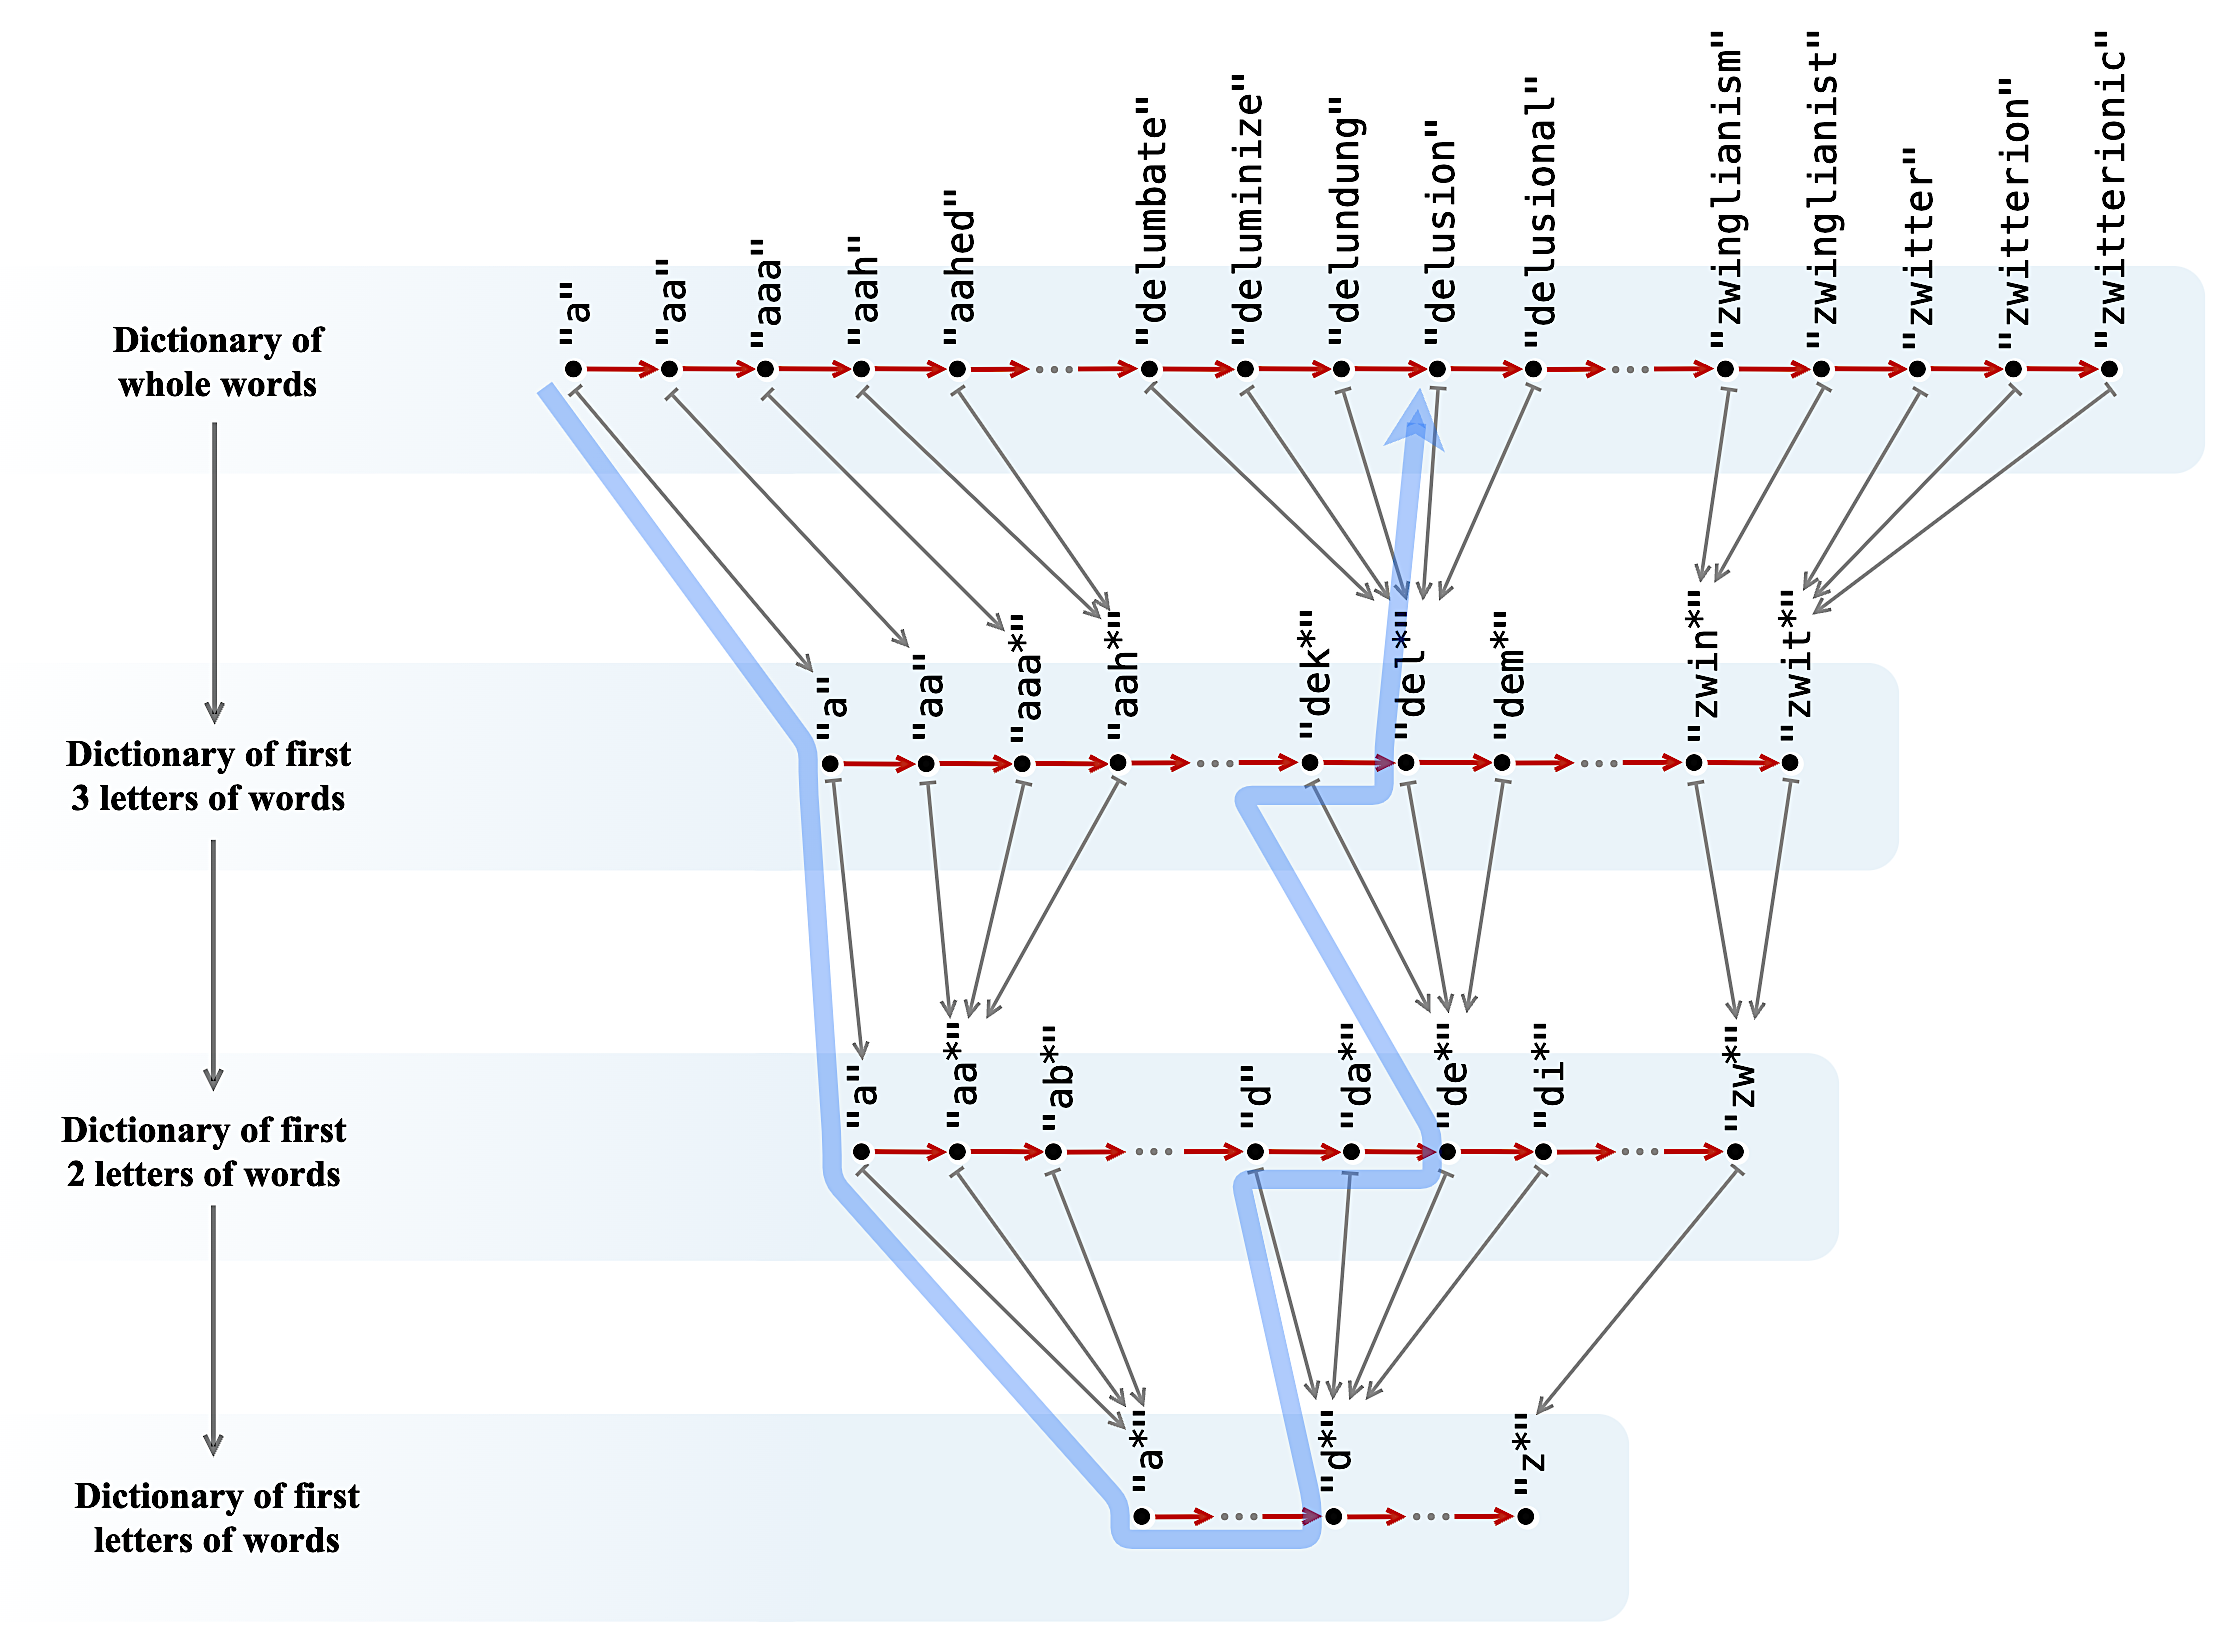
\includegraphics[scale=0.39]{../../assets/images/mathematical_model/dict_lookup.png}
    $$
    \vskip -.5cm
    \caption{Movement through a dictionary as a path endpoint problem organized by a prefix tower.  Prefixes are quotient addresses.}
    \label{fig:dictionary}
\end{figure}

HNSW implements an analogous address system geometrically: long-range edges at high levels give coarse addresses for a region of the point cloud, and lower levels refine that address by shorter local moves. Search therefore proceeds by descending through a hierarchy of increasingly fine neighborhoods, so the number of graph moves needed to localize a target scales logarithmically under the usual navigability assumptions.

We can also cast the logarithmic speed-up in terms of path specification. The hierarchy contracts long flat paths into short address paths. A path that would require specifying many primitive transitions in the base space can instead be specified by a small number of coarse choices followed by local refinements. The logarithm appears because each coarse address step represents a fixed-scale contraction of the remaining traversal distance.

Abdul Malik applied these ideas to graph ML learning in \cite{MalikThesis}. In Malik's work, a graph tower is used to organize simplex detection by passing from the original graph to a sequence of quotient graphs. Candidate simplex structure can then be searched for at coarser levels first and lifted back to finer levels only when necessary. The tower therefore acts as an addressing scheme for combinatorial structure in the graph, reducing the amount of flat graph search required before a promising local configuration is identified.
\end{example}

\begin{example}
{\bf U-Nets and ResNets.}
\normalfont

This intution, that putting a hierarchical structure on a computing problem can induce a logarithmic speed-up, is also hidden in the CNN architecture of U-Nets \cite{FB15} and ResNets \cite{HZRS15}, where it again induces a logarithmic improvement. 

Indeed, the speed-up provided by HNSW comes from an geometrically thinned hierarchy of coarsened spaces. The original HNSW paper describes the hierarchy as links separated by characteristic distance scale, enabling logarithmic complexity scaling. A U-Net does essentially the same thing: each downsampling layer reduces the number of sites and increases the physical scale represented by one feature. Thus, a U-Net is HNSW-like for spatial/frequency information flow.
\begin{figure}[!h]
	\vskip -.5cm
    $$
    \!\!\!\!\!\!\!\!
    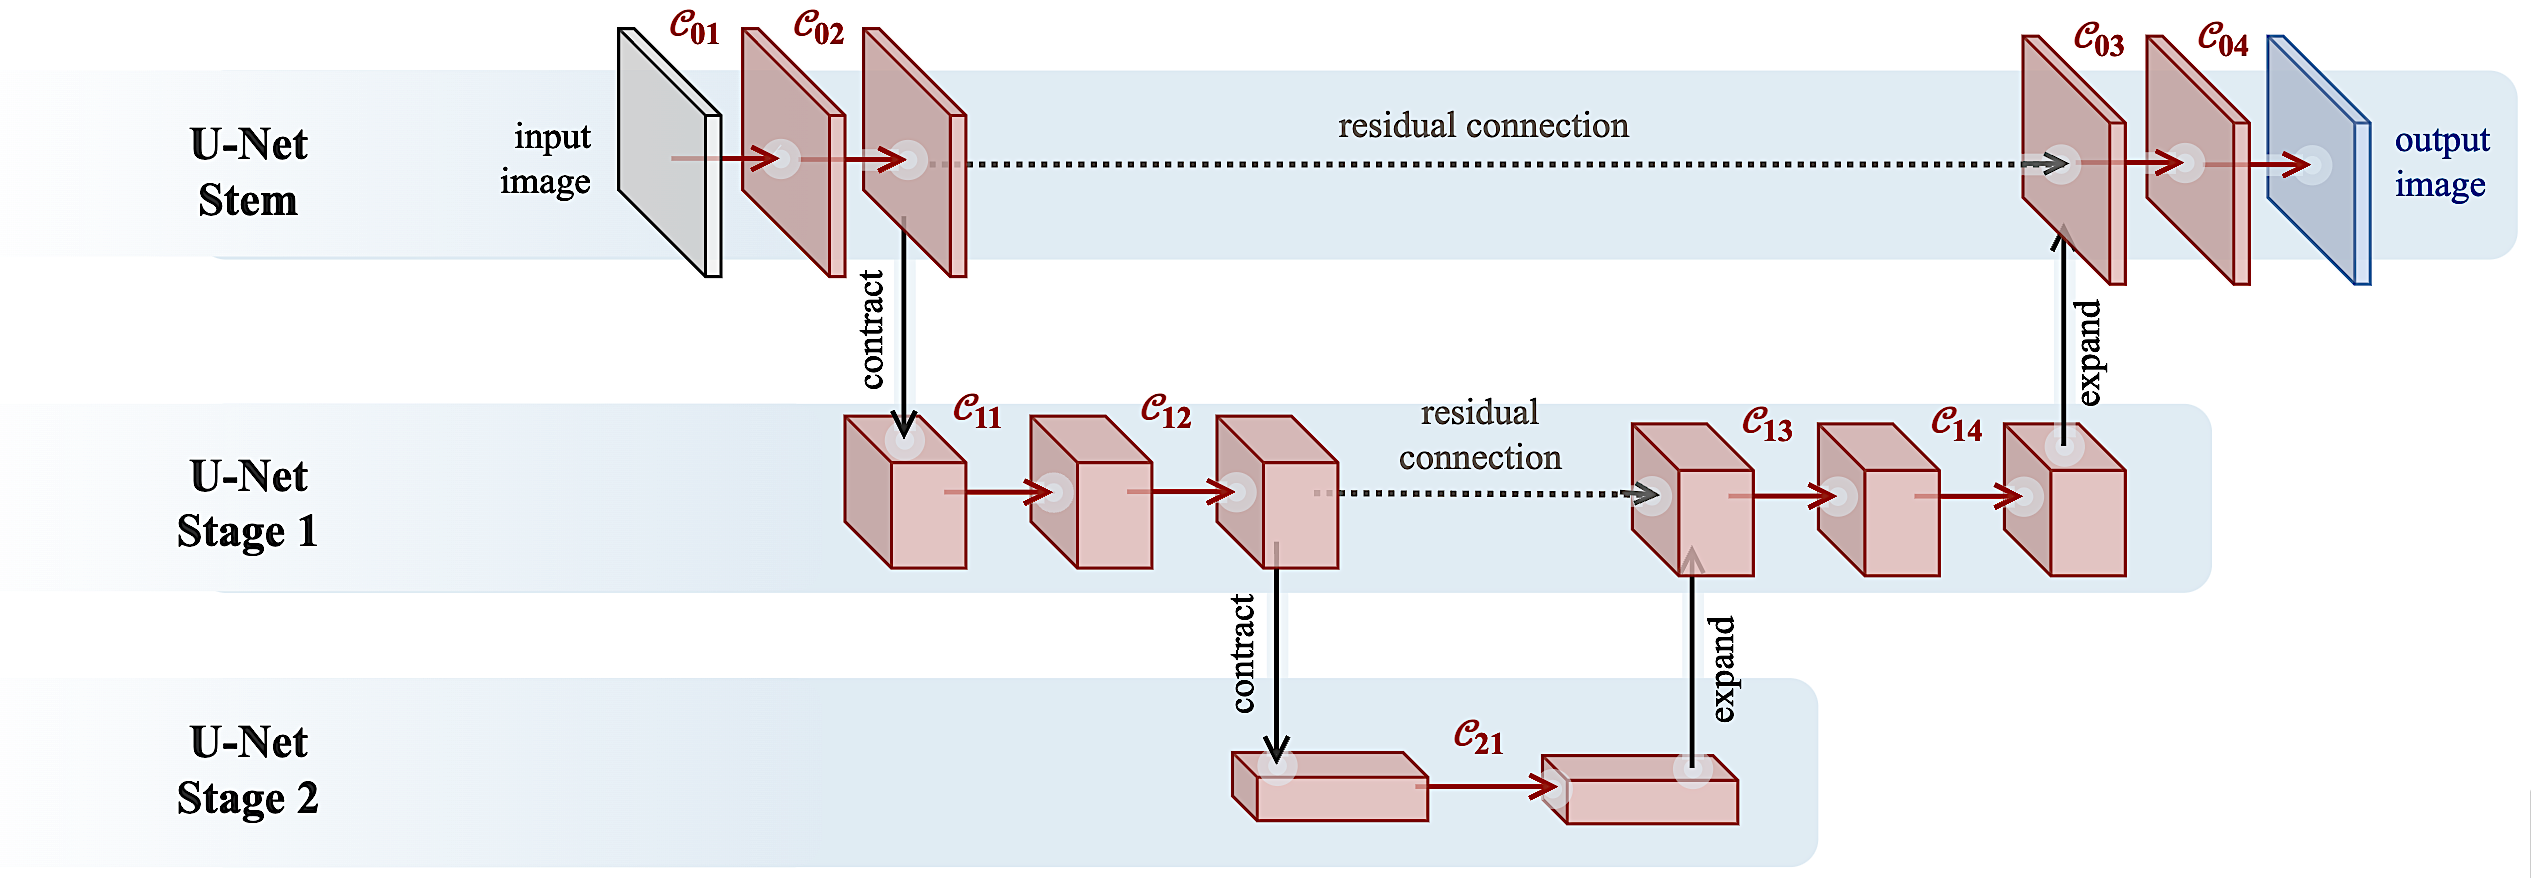
\includegraphics[scale=.37]{../../assets/images/mathematical_model/unet.png}
    $$
    \vskip -.5cm
    \caption{A U-Net-style multiscale architecture is best read here as an instantaneous/tangent analogue of a path space quotient tower}
\end{figure}

For residual correction, it is {\em multigrid}-like, in the sense of \cite{AhamedZakariaeiHaberEliasofMGE2026}. MgNet makes this correspondence especially explicit: restriction maps pass information to a coarser grid, smoothing operations remove local high-frequency error, and prolongation maps lift coarse corrections back to the fine scale. Read through this lens, a residual CNN is not merely a stack of feature extractors; it is also an iterative correction scheme in which coarse representations control the search for fine-scale residual structure.

When the training procedure/loss is itself is organized coarse-to-fine, the U-Net becomes HNSW-like for weight-space search as well, and we get a logarithmic speed-up in train time.
\end{example}

\begin{example}
{\bf Hints from hierarchical RL.}
\normalfont
Consider the RL problem of training a program to write Western tonal counterpoint by choosing the next chord an {\em a cappella} musical texture formed from $n$ voices. So for instance, in a string trio, $n=3$ and the voices are a violin, a viola, and a cello. In a barbershop quartet, $n=4$ and the voices are the lead, the tenor,  the baritone, and the bass.

Regardless of what the specific voices are, the combinatorics of next-chord choice explodes as the number of voices grows:
\begin{enumerate}
\item \vskip -.2cm
If the texture has one voice, then the agent is choosing a next note in a melody. If we restrict attention to locally plausible diatonic motion, for example repeated note, step up/down, and small skip up/down, then a reasonable working estimate is
$$
\mathbb{E}\big[\#\,\text{possible next notes}\big]\;\approx\;5
$$
If we understand melody writing as making a choice of ``next note'' over and over again, RL-style, then the number of possible melodies quickly explodes. For instance, with the above working estimate
\begin{figure}[!h]
	\vskip -.5cm
    $$
    \ \ \ \ \ \ \ \ \ \ \ 
    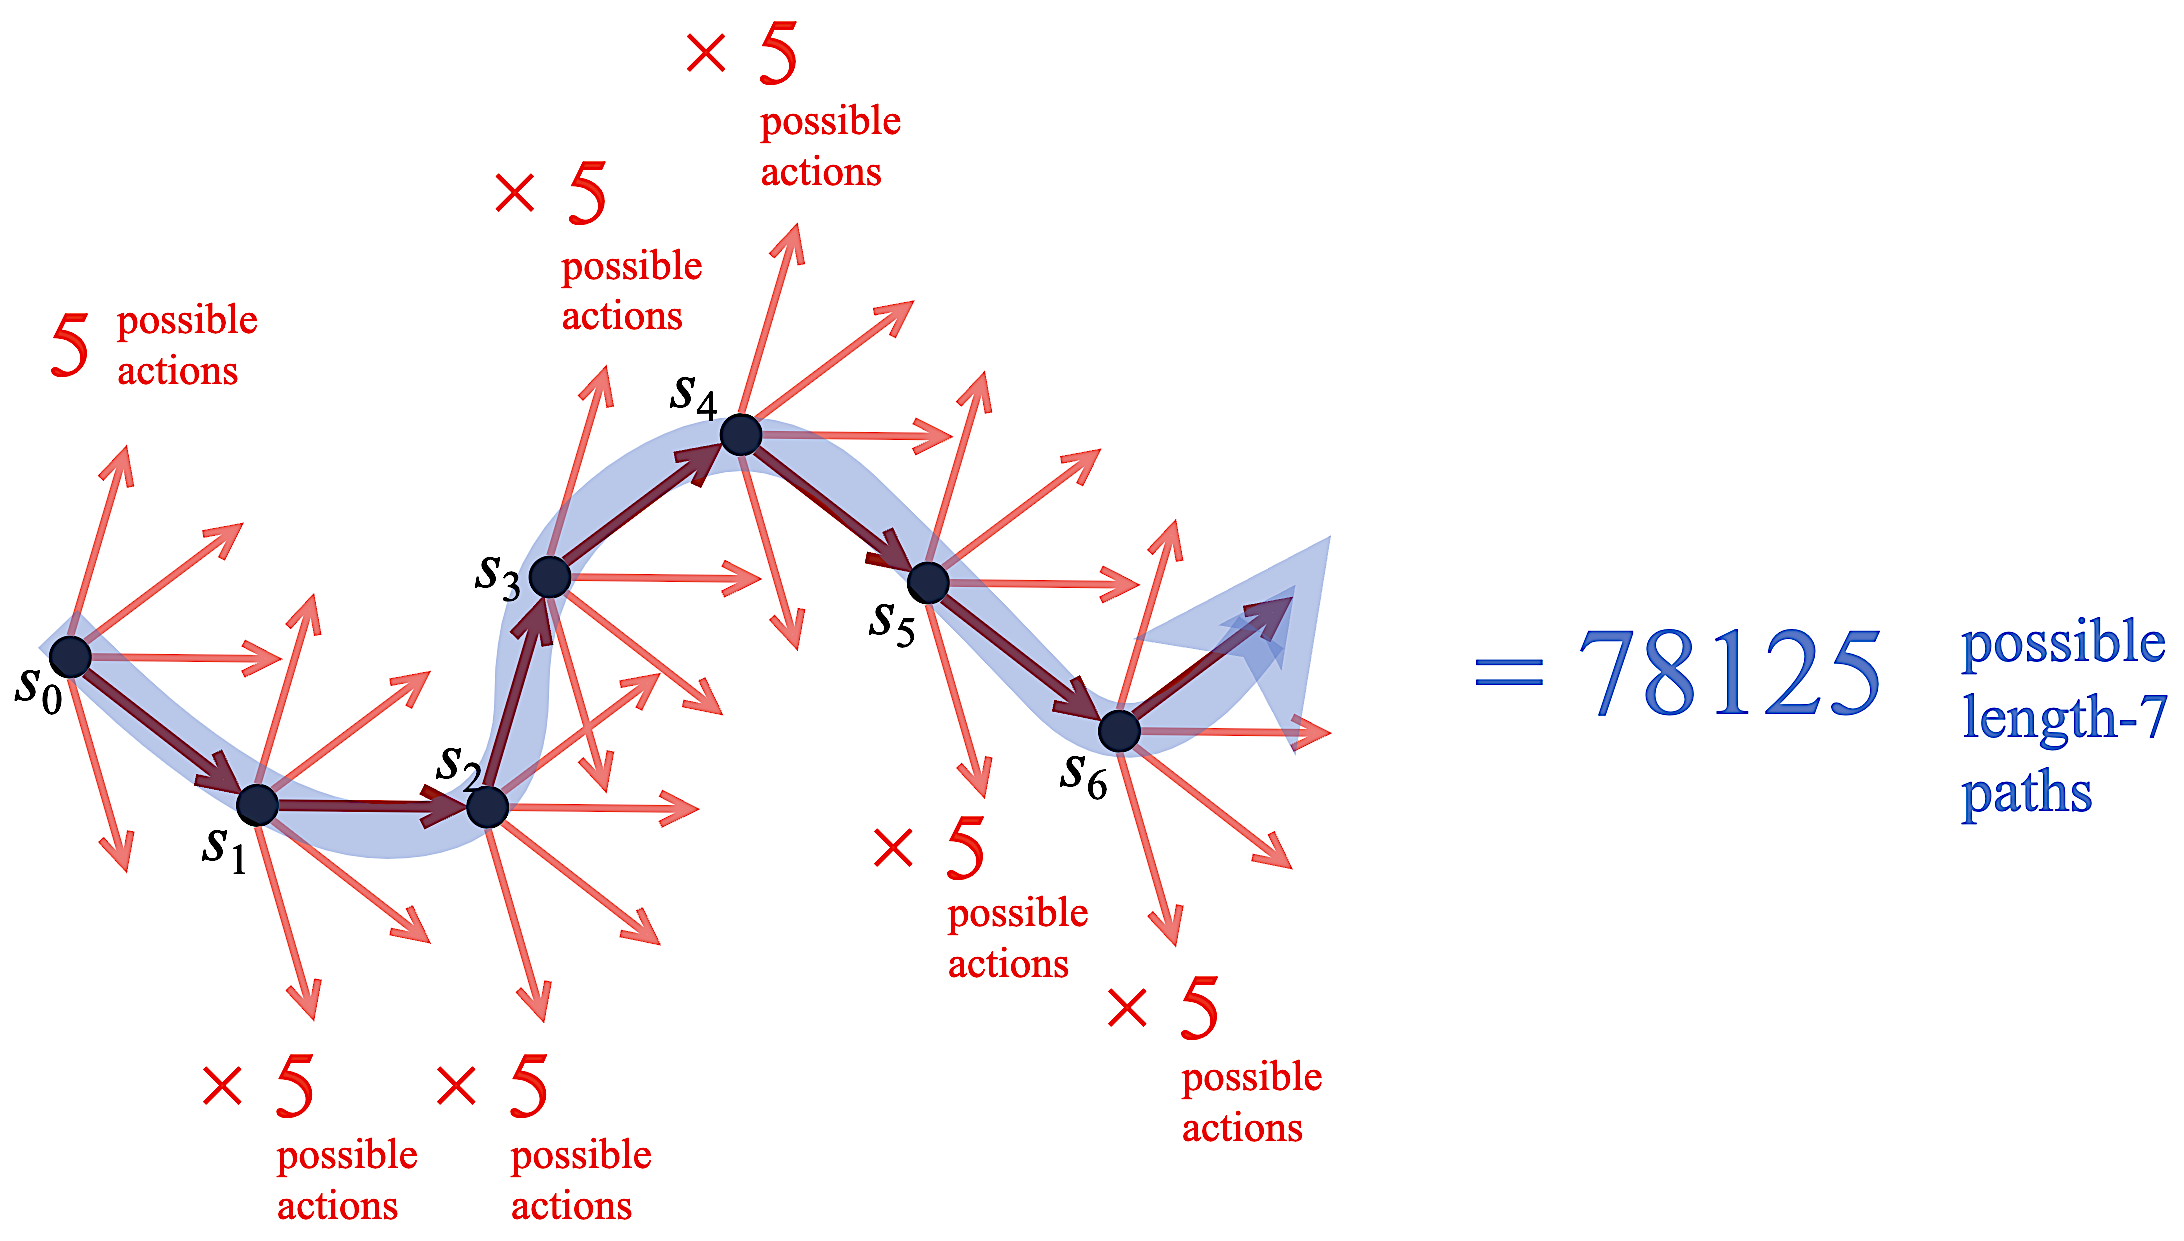
\includegraphics[scale=.3]{../../assets/images/mathematical_model/paths.png}
    $$
    \vskip -.5cm
    \caption{Making a choice among ``the next $5$ possibilities'' $7$ consecutive times leads to $78\,125$ possible sequences of choices, i.e., $78\,125$ possible paths.}
    \label{fig: possible paths}
\end{figure}
\item\vskip -.5cm
If the texture has two voices, then it is choosing a next interval, subject to voice-leading constraints like ``no parallel fifths'' and ``no crossing voices'.' As a rough local estimate, if each voice has about five plausible next pitches before cross-voice filtering, then there are about $5^2=25$ raw next intervals; after excluding voice crossing, spans over two octaves, and parallel fifths or octaves, a reasonable working estimate is
$$
\mathbb{E}\big[\#\,\text{possible next intervals}\big]\;\approx\;15
$$
\item\vskip -.2cm
If the texture has three voices, then it is choosing a next trichord, subject to voice-leading constraints. The raw local count is about $5^3=125$, but the three pairwise voice relations impose ordering, width, and parallel-perfect-interval exclusions; a useful rough estimate is
$$
\mathbb{E}\big[\#\,\text{possible next trichords}\big]\;\approx\;60
$$
\item\vskip -.2cm
If the texture has four voices, then it is choosing a next tetrachord, subject to voice-leading constraints. The raw local count is about $5^4=625$, and the six pairwise voice relations cut this down substantially, but not nearly enough to make the flat action space small; a conservative working estimate is
$$
\mathbb{E}\big[\#\,\text{possible next tetrachords}\big]\;\approx\;180
$$
\vskip -.2cm
\end{enumerate}
\begin{figure}[!h]
\vskip -.5cm
    $$
    \!
    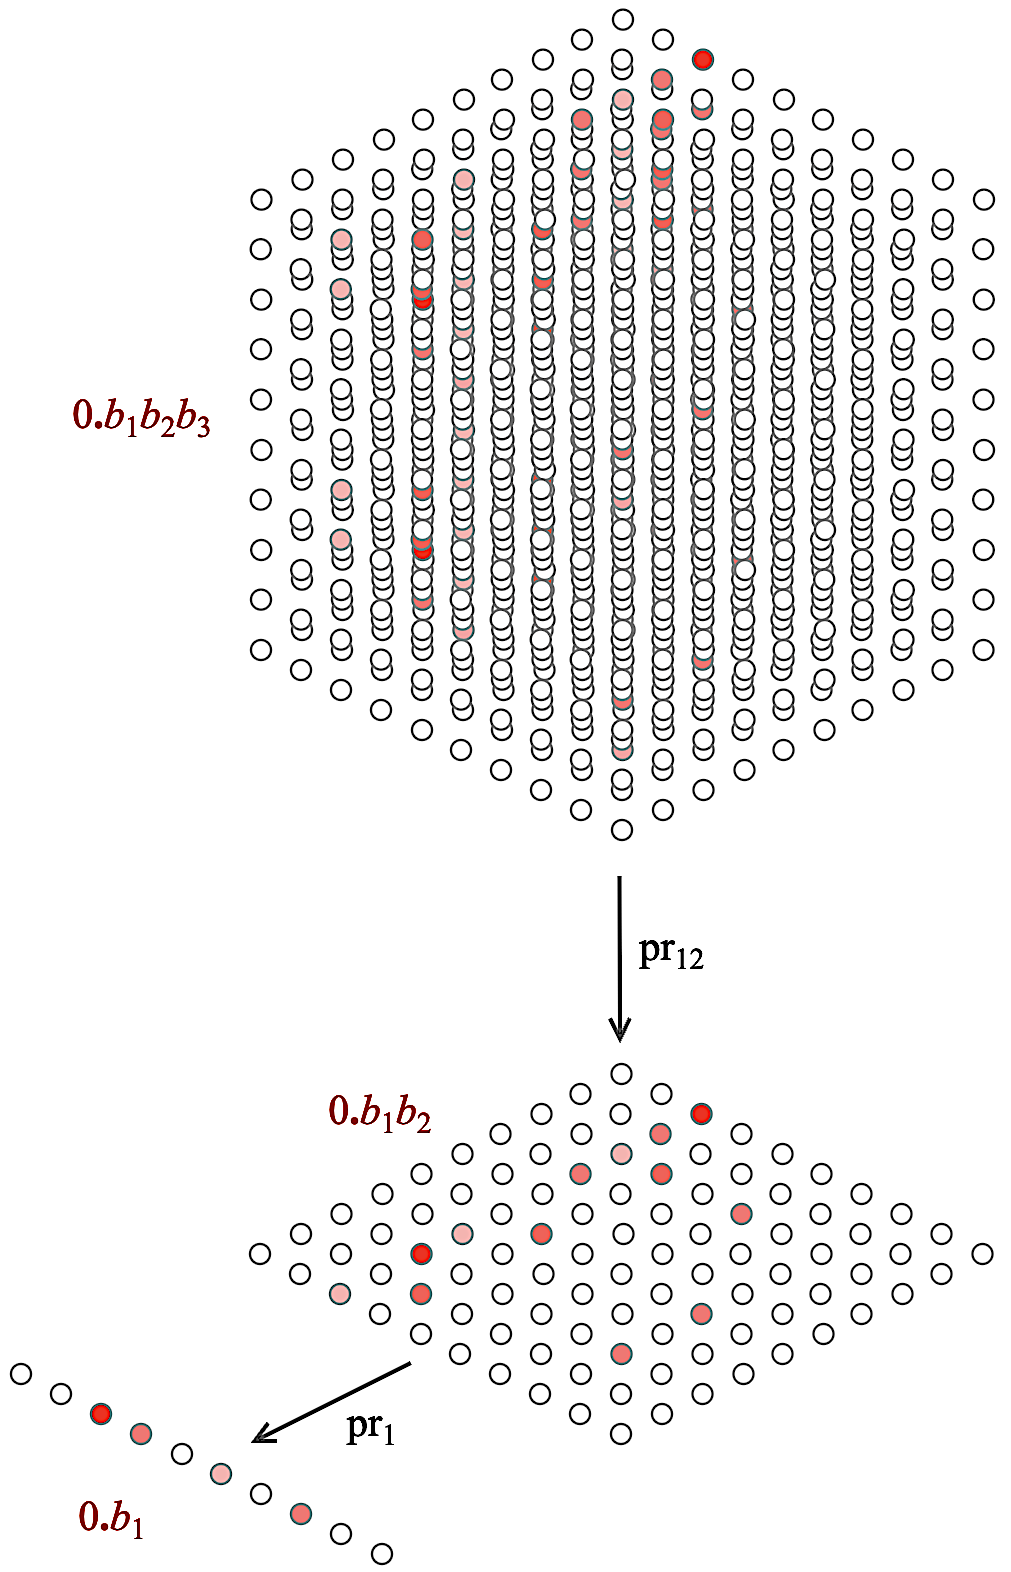
\includegraphics[scale=0.3]{../../assets/images/mathematical_model/sparse_base_10.png}
    \quad\quad\quad\quad
    \vline\vline\quad
    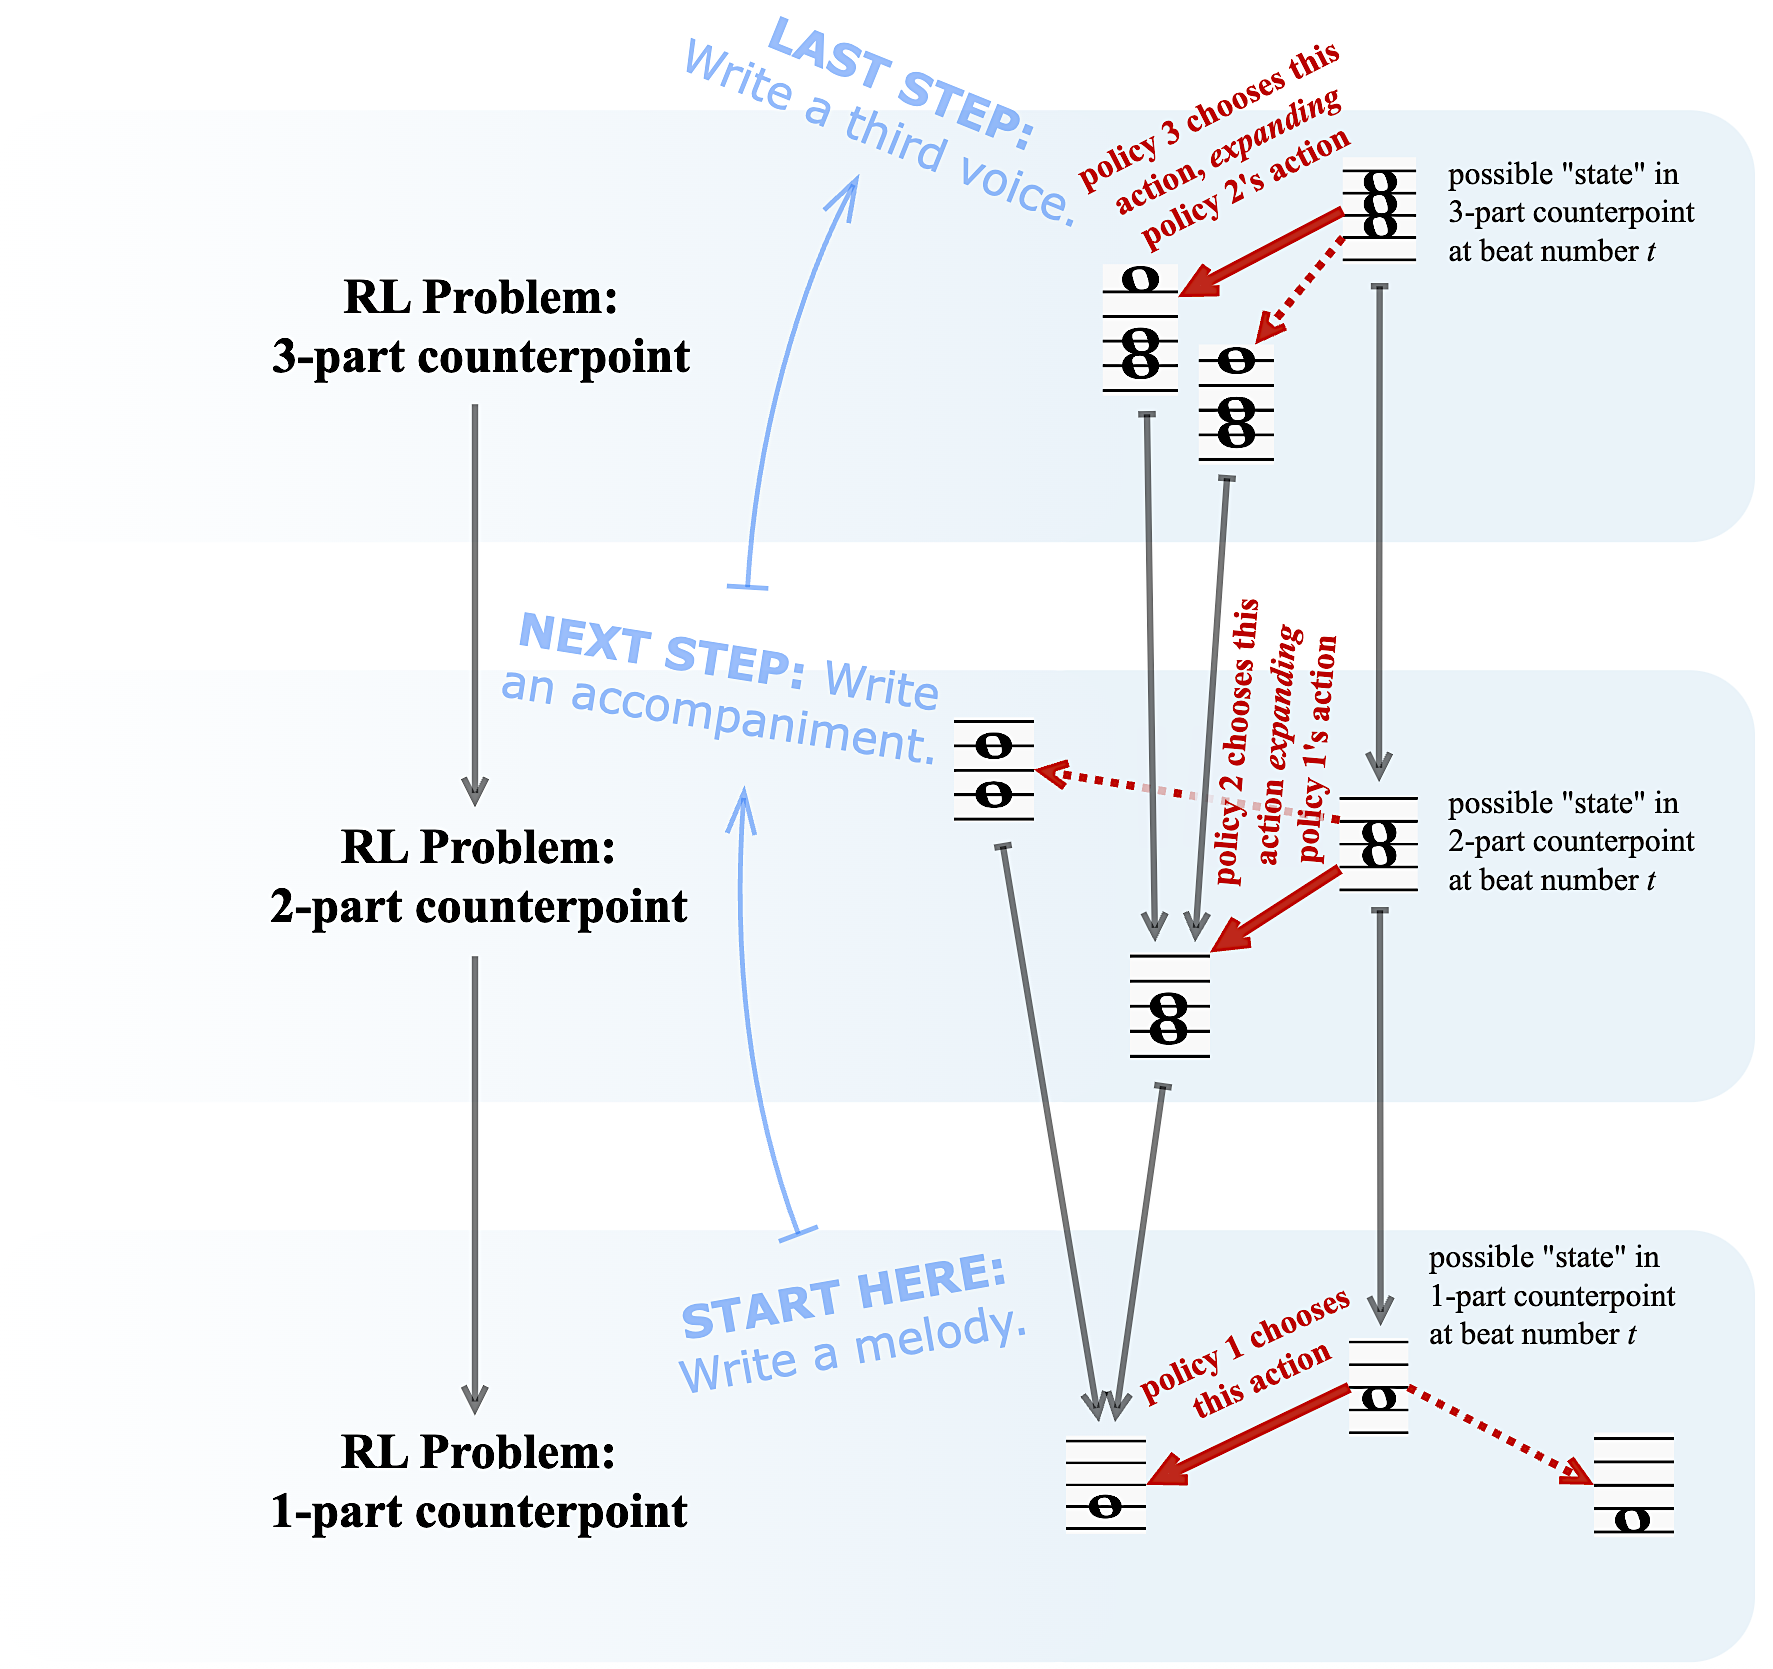
\includegraphics[scale=.3]{../../assets/images/mathematical_model/HRL_counterpoint.png}
    $$
    \vskip -.5cm
    \caption{(Left) A positional address system replaces flat enumeration by logarithmic-length descriptions. (Right) Counterpoint as staged path-space search: one-part melodic structure constrains two-part writing, which then constrains richer textures. The package does not require such a human-readable hierarchy, but this example explains why quotient hierarchy matters.}
    \label{fig: hierarchical paths}
\end{figure}
The number of plausible next actions grows very quickly with the number of voices, and the number of possible episodes grows exponentially with the length of the musical passage. Thus even before the reward function is subtle, the flat path space for ``next chord'' counterpoint is already enormous.

The agent is not merely choosing among a few next moves; it is searching through a huge space of possible voice-leading paths.

In practice, human musicians do not usually learn or write counterpoint by trying all voices at once until a good texture appears. They build the object hierarchically. One first learns to write a good melodic line. Then one learns to add a good accompanying line against it. Then one learns to fill in inner voices, decorations, suspensions, or harmonic support against an already constrained two-part skeleton. Each stage reduces the effective search problem for the next stage. Fixing or learning a melody first quotients out much of the full multi-voice texture space: the later voices are no longer searched against the entire path space of all possible chords, but against a structured lower-dimensional scaffold. The hierarchy is not just a musical convenience. It is an address system for path space, as depicted in Figure \ref{fig: hierarchical paths}.
\end{example}

\begin{example}
{\bf Difficulties in RL for coordinated movement.}
\normalfont
Coordinated movement problems are difficult because the useful action is rarely a single independent primitive. The agent must move several degrees of freedom in concert, and the reward signal often appears only after a coordinated path has been completed. This creates a flat search problem with a large combinatorial branching factor. A quotient tower helps by grouping coordinated families of primitive moves into abstract movement directions, so the agent can search over coarse coordinated addresses before refining to concrete actions.

For example, suppose a robot arm must move a box into a container in three-dimensional space. The flat state/action graph records all small coordinated motions of the arm, gripper, and box. But one quotient task is obtained by projecting away horizontal motion and retaining only height: first learn how the box should move in the $z$-direction as a function of time. Another quotient task is obtained by projecting to the floor: learn where the box must move in the $xy$-plane, temporarily ignoring its height. These projected problems are not subtasks in the sense of being independently executable pieces of the full task. They are quotient tasks: they collapse some degrees of freedom so that the control problem has a shorter address. The full policy can then be learned as a refinement that lifts these quotient policies back to coordinated motion in the original configuration graph.

\begin{question}
Why should the contractions in the quotient tower be required to be ideal?  As suggested by the graph HNSW speed in simplex search achieved in \cite{MalikThesis}, could one obtain the same logarithmic search effect from random or approximately balanced contractions, provided that reward descent and liftability hold only approximately?
\end{question}
\end{example}


\end{subsection}

\begin{subsection}{Main theorem: Problem agnostic, hierarchical log speed-up for RL train}

Suppose that the agent's explored state/action graph admits a quotient tower whose levels behave like an address system for the useful paths in the problem. Instead of searching directly through a flat set of primitive paths, the controller first chooses a coarse quotient address and then refines that choice through successive tiers until an executable primitive path is obtained. The theorem below records the idealized consequence of this situation: when the tower covers the relevant path space, rewards descend well enough through the quotients, and lifts back to executable actions are available, the flat search term can be replaced by a logarithmic address-search term plus the residual costs of lifting, refinement, and statistical estimation.

\begin{assumptions}\label{ass: simple ass}
Rewards are action-local after any necessary state augmentation, and quotient rewards are trained or estimated as direct-image reward aggregations on action cells. The aggregation rule is a modeling choice: sums, conditional expectations, maxima, soft maxima, or order-$p$ means/norms may be appropriate depending on whether the quotient task should preserve total, typical, best-case, or risk-sensitive fine behavior.
 

There are positive integers \(b_m,b_{m-1},\ldots,b_0\) and nonnegative residual terms \(\epsilon_i\) such that the tower controller can choose the coarsest address and each subsequent refinement with expected cost
$O(\log b_i)+\epsilon_i$, with induced address capacity $\prod_{i=0}^{m} b_i \ge |G^{0}_{t}|$.
When the tower is approximately balanced, the product is of the same order as \(|G^{0}_{t}|\).
\end{assumptions}


\begin{theorem}\label{theorem: main}
Suppose Assumptions \ref{ass: simple ass} hold.  Then the tower controller has search cost bounded by
$$
    \cost_{\mathcal{T}}(\Omega)
    \quad\le\quad
    C\sum_{i=0}^{m}\log b_i \;+\; \sum_{i=0}^{m}\epsilon_i
$$
for a model-dependent constant \(C\), providing a logarithmic improvement lat search over \(\Omega\), which has has enumeration cost $
    \cost_{\mathrm{flat}}(\Omega)=\Theta(|\Omega|)=\Theta(\PVol_{\Omega}),
$
where \(\PVol_{\Omega}=|\Omega|\) is the finite path volume of the relevant path set.  In the balanced case, where \(\prod_i b_i\asymp |\Omega|\), this becomes
$$
    \cost_{\mathcal{T}}(\Omega)
    =O\bigl(\log \PVol_{\Omega}\bigr)+\sum_{i=0}^{m}\epsilon_i.
$$
\end{theorem}

\end{subsection}

\begin{subsection}{Main Corollary: The \texttt{state\_collapser} package}

Our main corollary puts our theorem into production. It says that an efficient implementation of our tier-constructing mathematical model can provide logarithmic speed-up for RL training.

\begin{ermark}
{\bf The \texttt{state\_collapser} package.}
\normalfont
The mathematics below describe a robust, abstract strategy for inducing an HRL structure on RL problems that have no canonical or intrinsic hierarchical structure. We claim, in this document, to see how to induce HRL structures where there aren't any.

To deliver on our claims in a way that engineers can appreciate and can maybe even deploy in production, we've developed the Python package \texttt{state\_collapser}.
\begin{quote}
{\sf
\textsf{\textbf{Package name:}} \texttt{state\_collapser}

\textsf{\textbf{Package description:}} A Python package for inducing hierarchical RL structure on RL problems with {\em no} obvious subtask decomposition or natural human-readable hierarchy.

\textsf{\textbf{Repo link:}}  \href{https://github.com/TYLERSFOSTER/state_collapser}{\externallink\;\texttt{TYLERSFOSTER/state\_collapser}}

}
\end{quote}

\noindent
Making no assumption that there is any hierarchy visible in a given RL problem specification, the \texttt{state\_collapser} package constructs quotient-style tower structure by recursively contracting discovered state/action-graph structure. The result is a runtime layer for coarse-to-fine HRL control that navigates intermediate, state/action graphs wherein states and actions have been ``collapsed'', and are not be directly executable, but can be refined or ``lifted'' to executable executable behavior.

The payoff is a reduction in effective search and training burden. Rather than repeatedly learning over the full, ``fine-scale'' path space associated to the original RL problem, the agent can learn first over more collapsed quotient structure, then return to finer tiers only for the additional correction that the coarser tiers could not supply. In the best case, this replaces broad flat exploration with staged coarse-to-fine control over a much smaller effective path space.
\end{ermark}

\begin{corollary}[{\bf Problem agnostic, hierarchical log speed-up for RL train}]\label{cor:state-collapser}
If the runtime contractions produced by \texttt{state\_collapser} generate a quotient tower satisfying coverage, action-local reward descent, liftability, and balanced addressability for the path set actually explored by training, then the package replaces the flat path space search term \(\Theta(\PVol)\) by a quotient-tower search term of order
\[
    O(\log \PVol)+\text{lift/refinement/statistical residuals}.
\]
\end{corollary}

\end{subsection}

\end{section}


\vskip .5cm
\begin{section}{Underlying formulations of RL and HRL}

We will try to follow the notation in \cite[pp. xix-xxii]{SBRL}. That said, we {\em will} deviate from that book's notation when it serves out purposes.

\begin{subsection}{Standard formulation of RL}

\begin{ermark}
{\bf Three curtains.}
\normalfont
We want to distinguish three layers that are often conflated in informal discussions of RL. 
\begin{enumerate}
\item
The {\em real system} or {\em real world}, which may contain far more structure than the learner ever observes. 
\item
The {\em environment model} presented to the agent. These are the state/action interface, transition mechanism, and reward mechanism through which the real system is made computationally accessible. 
\item
{\em The agent's internal training representation}, which may replace concrete states by histories, observations, quotient cells, or learned features. 
\end{enumerate}
This project exist in the second and third layers. The quotient tower we build is a structured computational representation through which the agent can move more efficiently.
\end{ermark}

We now fix the formal state/action language used for the environment model. The definitions in this subsection are intentionally elementary: states are nodes, primitive actions are directed edges, and histories are paths. This gives us a concrete graph-theoretic object on which policies, rewards, rollout distributions, and eventually quotient towers can all be defined.
 
\begin{definition}
\normalfont
A finite directed {\em state/action-graph} $H$ is a finite directed graph
\begin{equation}\label{eq:H src tgt}
H\;\quad=\quad\;
\begin{xy}
(0,0)*+{\mathcal{A}_{H}}="1";
(20,0)*+{\mathcal{S}_{H}}="2";
{\ar@<2pt>^{\text{tgt}} "1"; "2"}
{\ar@<-2pt>_{\text{src}} "1"; "2"}
\end{xy}
\end{equation}
where $\mathcal{S}_{H}$ is the set of all possible states of some system we're interested in, and $\mathcal{A}_{H}$ is the set o all possible primitives actions between any two of the states in our system, meaning that every action in $\mathcal{A}_{H}$ transpires over a fixed time interval, for time step $t$ to time step $t+1$.

Given a state $s\in\mathcal{S}_{H}$, we let $\mathcal{A}_{H}(s)\subset \mathcal{A}_{H}$ denote the set of all outgoing actions at $s$, this is, that set of all $\alpha\in\mathcal{A}_{H}$ such that
$\text{src}(\alpha)=s$. In terms of the graph $H$, we can characterize $\mathcal{A}_{H}(s)$ as the edge set of the outgoing 1-hop neighborhood of $s$ in the state/action-graph $H$.
\end{definition}

\noindent
We will return to the following two examples several times. They represent two computational depictions, or encodings of the same physical system, where states are simply positions in some rectilinear region
$$
\text{Room}
\;:=\;
[0,\,\ell_1]\times[0,\,\ell_2]\times[0,\,\ell_3]\;\subset\;\mathbb{R}^{3},
$$
with volume $\text{Vol}(\text{Room})=\ell_{1}\ell_{2}\ell_{3}$

\begin{example}\label{ex: actions match projections}
{\bf Region of 3-dimensional space as la grid lattice:}
\normalfont
Suppose the RL problem's hidden state space $\mathcal{S}_{H}$ is just some region in $\mathbb{R}^{3}$ discretized as a fine grid
$$
\mathcal{S}_{H}
\;=\;
\Big\{(i\Delta x,\,j\Delta y,\,k\Delta z)\in\mathbb{R}^{3}:
0\le i\le N_1,\;
0\le j\le N_2,\;
0\le k\le N_3
\Big\}
$$
At each interior point, the possible actions are to add or subtract one mesh width unit $\Delta x$, $\Delta y$, or $\Delta x$ in the respective direction:
$$
\scalebox{.8}{$
\pmb{
\begin{xy}
(0,0)*+{(x,\,y,\,z)}="000";
(35,-10)*+{(x+\Delta x,\,y,\,z)}="100";
(-35,10)*+{(x-\Delta x,\,y,\,z)}="-100";
(35,10)*+{(x,\,y-\Delta y,\,z)}="010";
(-35,-10)*+{(x,\,y+\Delta y,\,z)}="0-10";
(0,30)*+{(x,\,y,\,z+\Delta z)}="001";
(0,-30)*+{(x,\,y,\,z-\Delta z)}="00-1";
{\ar^{+\Delta x} "000"; "100"};
{\ar^{+\Delta y} "000"; "010"};
{\ar_{+\Delta z} "000"; "001"};
{\ar_{-\Delta x} "000"; "-100"};
{\ar_{-\Delta y} "000"; "0-10"};
{\ar_{-\Delta z} "000"; "00-1"};
\end{xy}
}
$}
$$
At boundary states, meaning positions on the boundaries of the enclosed region, some subset of these actions will be missing.

One critical feature of this examples is that natural projections $\text{pr}_{xy},\,\text{pr}_{yz},\,\text{pr}_{xz}:\mathbb{R}^{3}\longrightarrow\mathbb{R}^{2}$ to coordinates planes and projections $\text{pr}_{x},\,\text{pr}_{y},\,\text{pr}_{z}:\mathbb{R}^{3}\longrightarrow\mathbb{R}$ to coordinate axes, which come from the ambient geometry in this example, induce natural quotient morphisms of $H$. For instance
$$
\text{pr}_{yz}:\mathbb{R}^{3}\longrightarrow\mathbb{R}^2
\;\;\text{induces quotient morphism}\;
\begin{xy}
(0,0)*+{H}="1";
(27,0)*+{H\!\big/\{x\text{-axis actions}\}}="2";
{\ar@{->>} "1"; "2"};
\end{xy}
$$
and
$$
\text{pr}_{x}:\mathbb{R}^{3}\longrightarrow\mathbb{R}
\;\;\text{induces quotient morphism}\;
\begin{xy}
(0,0)*+{H}="1";
(33,0)*+{H\!\big/\{y\text{- and }z\text{-axis actions}\}}="2";
{\ar@{->>} "1"; "2"};
\end{xy}.
$$
\end{example}


\begin{example}\label{ex: point cloud}
{\bf Region of 3-dimensional space as a point cloud:}
\normalfont
Take the same region $[0,\,\ell_1]\times[0,\,\ell_2]\times[0,\,\ell_3]\subset\mathbb{R}^{3}$, but now let $\mathcal{S}_{H}$ be a set of $(N_{1}+1)(N_{2}+1)(N_{3}+1)$ points sampled i.i.d. uniformly from $[0,\,\ell_1]\times[0,\,\ell_2]\times[0,\,\ell_3]$. This sampling gives us a {\em point density}
$$
\rho_{H}\,=\,\frac{\#\mathcal{S}_{H}}{\ \text{Vol}(\text{Room})\ }
$$
Fix the {\em connectivity threshold}
$$
\delta_{H}
\;:=\;
\left(
\frac{9}{4\pi\rho_{H}}
\right)^{\!1/3},
$$
and declare that there are actions
$$
\begin{xy}
(0,0)*+{(x_{1},\,y_{1},\,z_{1})=:\bold{r}_{1}}="1";
(45,0)*+{\bold{r}_{2}:=(x_{2},\,y_{2},\,z_{2})}="2";
{\ar@<2pt>^{\alpha^{1}_{2}} "1"; "2"}
{\ar@<2pt>^{\alpha^{2}_{1}} "2"; "1"}
\end{xy}
$$
present in the state/action graph $H$ precisely when
$$
\text{dist}(\bold{r}_{1},\,\bold{r_{2}})
\;\le\;\delta
$$
Unlike Example \ref{ex: actions match projections},  each of the coordinate plane projections $\text{pr}_{xy},\,\text{pr}_{yz},\,\text{pr}_{xz}:\mathbb{R}^{3}\longrightarrow\mathbb{R}^{2}$ and coordinate axis projections $\text{pr}_{x},\,\text{pr}_{y},\,\text{pr}_{z}:\mathbb{R}^{3}\longrightarrow\mathbb{R}$ will tend not to identify any of our sampled points in $\mathbb{R}^{3}$, and so will not induce a map to a smaller quotient graph.
\end{example}

\begin{remark}
{\bf Terminal states.}
\normalfont
Sutton and Barto are careful to distinguish between arbitrary states and {\em terminal} states, meaning terminal states $s$ with no outgoing actions. In the present note, we let $\mathcal{S}_{H}$ denote {\em all} possible states, including terminal states.
\end{remark}

\begin{remark}
{\bf The state/action-graph is {\em hidden}.}
\normalfont
One should understand the state/action-graph as representing the space of all possible configurations our system mind end up in. In practice, when confronted with a given system, we initially don't know much about possible configurations the system could be in, and what actions are possible. We map out the possible states of the system and actions between the states through a process of exploration and note taking as we do so.

So the agent traverses the hidden state/action-graph $H$, recording details of what it sees in memory or in some database as it does so.
\end{remark}

\begin{definition}
\normalfont
A {\em history} in $H$ is any graph homomorphism
$$
\gamma:\;\left(\underset{0}{\bullet}\xrightarrow{\ \ 1\ \ }\underset{1}{\bullet}\xrightarrow{\ \ 2\ \ }\cdots\underset{k-1}{\bullet}\xrightarrow{\ \ k\ \ }\underset{k}{\bullet}\right)
\;\xrightarrow{\ \ \ \ \ \ \ }\;H
$$
We will often describe a history $\gamma$ in $H$ by sequence of states and actions in its image, by writing
\begin{equation}\label{eq: general history}
\gamma\;=\;\left(s_{0}\xrightarrow{\ \ \alpha_{1}\ }s_{1}\xrightarrow{\ \ \alpha_{2}\ }\cdots\xrightarrow{\ \alpha_{k-1}\ }s_{k-1}\xrightarrow{\ \alpha_{k}\ }s_{k}\right).
\end{equation}
We will also refer to a history in $H$ as a {\em path} in $H$.

	The {\em path space} of $H$, denote $\bold{Path}(H)$, is the set of all histories, of all lengths, starting at all nodes of $H$. For a given nonnegative length $k$, we let $\bold{Path}_{k}(H)$ denote the set of all length-$k$ paths in $H$, starting at all nodes of $H$.
\end{definition}

\begin{remark}
{\bf Decompoistions of path space.}
\normalfont
The path space of $H$ is the discrete analogue of the usual topological path space $\Path(X):=C^0([0,1],X)$ associated to a topologicla space $X$

Note that $\bold{Path}_{0}(H)\cong\mathcal{S}_{H}$, the set of nodes of $H$, and that $\bold{Path}_{1}(H)\cong\mathcal{A}_{H}$

Thus the state/action graph $H$ can be recovered as the first two layers of its path space: length-$0$ paths are states, and length-$1$ paths are actions. Longer paths should be thought of as higher-order rollout data built from this same state/action grammar.

Purely in their capacity as sets, we have the decomposition
$$
\bold{Path}(H)\;=\;\bigsqcup_{k=0}^{\infty}\bold{Path}_{k}(H),
$$
which we can also write as
$$
\bold{Path}(H)
\quad\cong\quad
\mathcal{S}_{H}\;\sqcup\;\mathcal{A}_{H}\;\sqcup\;\bold{Path}_{2}(H)\;\sqcup\;\bold{Path}_{3}(H)\;\sqcup\;\cdots
$$
We extend the action source and target maps \eqref{eq:H src tgt} in $H$ to {\em path} or {\em history source} and {\em target} maps
$$
\begin{xy}
(0,0)*+{\!\!\!\!\!\!\!\!\!\!\!\!\!\!\!\bold{Path}(H)}="1";
(20,0)*+{\mathcal{S}_{H}}="2";
{\ar@<2pt>^{\text{tgt}} "1"; "2"}
{\ar@<-2pt>_{\text{src}} "1"; "2"}
\end{xy}
$$
\end{remark}

\begin{ermark}
{\bf Control and policy.}
\normalfont
Following the standard RL convention, a Markov policy on $H$ is a stochastic kernel
$
\pi:\mathcal{S}_{H}\longrightarrow\mathcal{P}(\mathcal{A}_{H})
$
such that the distribution $\pi(-|s)$ is supported on the outgoing action set $\mathcal{A}_{H}(s)$. Thus the policy assigns to each state a probability distribution on the local fiber of admissible actions above that state. In the quotient constructions below, this support condition is deliberately loosened: an abstract state-cell may use action information pooled across several representatives, so the policy becomes uniformized over a coset rather than tied to one concrete tangent fiber. In this limited sense, the policy has a microlocal flavor: it is a rule on the local outgoing directions at a state, and quotienting replaces pointwise local direction data by direction data attached to a neighborhood or coset.

There are two standard ways to display this dependence, depending on what information the policy is allowed to read. The first is the Markov or last-state version, where the policy sees only the current state. The second is the history-based version, where the policy sees the entire rollout so far, or some observation extracted from it:
\begin{itemize}
\item
Last state' based':
$$
\begin{array}{rrcl}
\pi_{\theta}:
&\mathcal{S}_{H}
&
\!\!\!\!\longrightarrow\!\!\!\!
&\mathcal{P}(\mathcal{A}_{H}\mid\mathcal{S}_{H}) \\[5pt]
&
s
&
\!\!\!\!\longmapsto\!\!\!\!
& \pi_{\theta}(-\mid s)
\end{array}
$$
\item
Full history based:
$$
\begin{array}{rrcl}
\pi_{\theta}:
&\bold{Path}(H)
&
\!\!\!\!\longrightarrow\!\!\!\!
&\mathcal{P}\Big(\mathcal{A}_{H}\Big|\text{out}\big(\bold{Path}(H)\big)\Big) \\[7pt]
&
\gamma
&
\!\!\!\!\longmapsto\!\!\!\!
& \pi_{\theta}\big(-\mid \text{out}(\gamma)\big)
\end{array}
$$
\end{itemize}
\end{ermark}

\begin{ermark}
{\bf The types of RL problems we consider here.}
\normalfont
We will consider RL problems that can be formulated in the following way.

\begin{quote}
{\bf Basic setup.}
An agent moves through the state/action-graph $H$, occupying a single state $s_{t}\in\mathcal{S}_{H}$ at each time step $t$, and traveling along a single edge 
$
s_{t}\xrightarrow{\ \ \alpha\ \ }s_{t+1}
$
in the interval from time step $t$ to time step $t+1$, for some action $\alpha\in\mathcal{A}_{H}$ with source state $\text{src}(\alpha)=s_{t}$.

The agent is rewarded and/or penalized for its actions as it travels through state space. {\em Solving} a given RL problem means coming up with some kind of policy that controls the agent's movement through state/action-space, such that 
\end{quote}
In this paper, such a policy will be represented by a stochastic kernel $\pi$ that assigns probabilities to admissible next actions, either from the current state alone or from whatever history/observation the learner is allowed to use. When no ambiguity is important, we write this in the Markov form $\pi(-|s)$. When the dependence on rollout history matters, we allow $\pi$ to be evaluated on a history or on an observation extracted from that history.
\end{ermark}
 
 \begin{ermark}
{\bf Cummulative local rewards.}
\normalfont
Some of our results below concern only movement of the agent through the state/action-graph. For these results, we can ignore the specific structure of the rewards the agent receives. 

For our results concerning logarithmic speed-up for RL training, on the other hand, we need to impose conditions on these rewards that ensure they have the ability to ``descend'' down hierarchies of RL problems. Fortunately for our purposes, the types of rewards we need are very common in RL problems where the policy $\pi(\alpha|s)$ consists of actions sampled stochastically from the output distribution of a backpropagation-trainable model $\mathcal{M}$
 \end{ermark}

\begin{remark}
{\bf }
\normalfont
We use the language of stochastic kernels, ie.., conditional probabilities, to describe the rewards an agent receives as it traverses an RL environment. All the key ideas in this paper are already at play in the special case that all reward sampling processes are deterministic, so that reward distributions and reward kernels become reward values and reward functions, respectively.

We add this extra layer of complexity because {\em it more closely resembles the way rewards occur or are implemented in real world RL problems}. In real life, most identifiable states of a system do not come with a deterministic reward. Most rewards in real life depend on a huge number of external parameters to the state of the particular system we're interested in a given RL problem.
\end{remark}
 
 \begin{definition}[{\bf Rewards for actions}]
 \normalfont
By a {\em reward distribution} associated to a given action $\alpha\in\mathcal{A}_{H}$, we mean a probability distribution $P_{\!\alpha}$ on the real number line $\mathbb{R}$ and some process that samples from it:
$$
r\;\sim\;P_{\!\alpha}
$$
\end{definition}

\begin{remark}
{\bf Reward distributions as reward values.}
\normalfont
When the distribution $P_{\!\alpha}$ is a Dirac delta supported at some point $r\in\mathbb{R}$, we can understand the {\em reward associated to} $\alpha$ as being the deterministic assignment of the reward value $r$ to the action $\alpha$:
$$
a\;\mapsto\;r(\alpha)
$$
\end{remark}

\begin{definition}[{\bf Action-local reward kernel}]
An {\em action-local reward kernel} on $H$ is a stochastic kernel, i.e., conditional probability
$$
P_{(-)}:\mathcal{A}_{H}\longrightarrow \mathcal{P}(\mathbb{R})
$$
that associates a probability distribution $P_{\alpha}$ to every action $\alpha\in\mathcal{A}_{H}$.
\end{definition}

\begin{remark}
{\bf Rewards kernels as reward functions.}
\normalfont
When every one of these distributions $P_{\!\alpha}$ is a Dirac delta supported at some point $r(\alpha)\in\mathbb{R}$, we can understand the action-local stochastic kernel as a {\em action-local reward function}
$$
r(-):\mathcal{A}_{H}\longrightarrow\mathbb{R}
$$
\end{remark}

\begin{definition}[{\bf Cumulative reward kernel}]
A {\em cumulative reward kernel} on histories in $H$ is a stochastic kernel
$$
P_{(-)}:\bold{Path}(H)\longrightarrow \mathbb{R}
$$
such that:
\begin{enumerate}
\item
The restriction of $P_{(-)}$ to $\mathcal{A}_{H}\cong\bold{Path}_{1}(H)\subset\bold{Path}(H)$ is an action local reward kernel.
\item
There exists some sequence $w_{\bullet}=(w_{0}, \;w_{1},\;w_{2},\;\cdots)$ of {\em decay weights} $w_{i}\in\mathbb{R}_{\ge0}$, such that for any history $\gamma=(s_{0}\xrightarrow{\ \ \alpha_{1}\ }s_{1}\xrightarrow{\ \ \alpha_{2}\ }\cdots\xrightarrow{\ \alpha_{k-1}\ }s_{k-1}\xrightarrow{\ \alpha_{k}\ }s_{k})$, of any finite length $k$, its associated reward can be computed as the convolution product $r(\gamma)=w_{\bullet}\ast r(\alpha_{\bullet})$, i.e.,
$$
    P_{\gamma}\;\;=\;\;\sum_{i=0}^{k-1} w_{i}\,P_{\alpha_{k-i}}
$$
\end{enumerate}
\end{definition}

\begin{remark}
\normalfont
When every one of these distributions $P_{\!\alpha}$ is a Dirac delta supported at some point $r(\alpha)\in\mathbb{R}$, we can understand the action-local stochastic kernel as a {\em action-local reward function}
$$
r(-):\bold{Path}(H)\longrightarrow\mathcal{P}(\mathbb{R}),
$$
and the condition that the reward function be cumulative becomes the identity of reward values
$$
    r(\gamma)\;=\;\sum_{i=0}^{k-1} w_{i}\,r(\alpha_{k-i}).
$$
\end{remark}

\begin{remark}
\normalfont
Note that because $\mathcal{A}_{H}\subset\bold{Path}(H)$, we can interpret a cummulative reward kernel as some sort of free ``weighted convolutive extension of an action-local reward kernel to a reward kernel on full histories.''

Since $\bold{Path}_{0}(H)\cong\mathcal{S}_{H}$ is also included in the full path space, a reward kernel on $\bold{Path}(H)$ may also assign values to stationary histories. These can be interpreted as rewards for remaining at a state for one virtual step, or equivalently as rewards attached to formal loop or stay transitions. This does not mean that cycles in the environment are being ignored. Ordinary cycles are still paths built from nontrivial actions; the extra length-$0$ or stay data merely records the reward contribution of being at a state without taking a primitive move.
\end{remark}
 
\end{subsection}

\begin{subsection}{Alternative formulation of RL: {\em supervised ML with virtual rollout database}}

I want to rearrange your picture of RL for a moment.

You say ``there is an agent, containing enough of a mind that it can follow some policy that guides its behavior as it wandering around in an environment collecting rewards, modifying its policy where it sees fit.'' 

This makes it sound like a dynamic unsupervised learning problem. 

No, I say! It's not that at all! It's just the familiar old supervised ML problem.

\begin{ermark}
{\bf Policies as distributions on path space.}
\normalfont
A policy \(\pi_\theta\) assigns to each history, or to a chosen observation of that history, a probability distribution over admissible next actions. The state-based notation $\pi(-|s)$ is only the Markov special case. In general, the model may consume a history $\gamma$, an observation of a history, or a quotient-tower summary of a history, and then return a distribution on next admissible actions. The induced distribution on path space is therefore policy-dependent even when the displayed notation suppresses this dependence.
\[
    \mu_{\theta,k}\in \Delta\big(\bold{Path}_k(H)\big)
\]
over \(k\)-step histories.  A training run samples from these distributions and uses the resulting reward-labelled histories to update \(\theta\).
\end{ermark}

\begin{ermark}
{\bf Policies as models-plus-weights on a concrete mahcine}
\normalfont
If we want to take a materialist's perspective, our policy is {\em really} just some familiar old ML model, a DNN, or a transformer, or a U-NET, or whatever.  And we train this model in exactly the same way we always to: we repeatedly evaluate the model’s performance on some set of tasks, and we adjust the model, in response, via gradient backpropagation.

It’s really the same old thing. 
\end{ermark}

The only part of this whole situation that’s {\em really} different from vanilla ML is that for RL, our labelled training data is ``stored'' in a {\em virtual rollout database}, and that our strategy for taken entries from this database is different than for vanilla ML.

\begin{definition}[{\bf Virtual rollout database}]
\normalfont
For a fixed policy \(\pi_\theta\), horizon \(k\), and stochastic kernel $P_{(-)}:\bold{Path}_{\le k}(H)\longrightarrow\mathcal{P}(\mathbb{R})$, the {\em virtual rollout database}, denoted $\text{VRD}_{\theta,k}(H,R)$ is a triple  consisting of
\begin{enumerate}
\item {\bf Keys set:} Histories will serve as {\em keys}, so a key is any path $\gamma\in\bold{Path}_{\le k}(H)$
\item {\bf Query processor:} Given a key $\gamma\in\bold{Path}_{\le k}(H)$, the {\em query processor} returns the reward distribution
$$
P_{\gamma}\;\in\;\mathcal{P}_{\le k}(\mathbb{R})
$$
\item {\bf Value sampler:} Given a key $\gamma$ and the query processor's returned distribution $P_{\alpha}$, the {\em value sampler} samples a reward value from this distribution:
$$
r_{\gamma}\;\sim\;P_{\gamma}
$$
\end{enumerate}
The database is {\em virtual} in the sense that the triples $(\gamma,P_{\gamma},r_\gamma)$ that result from queries to it aren't actually stored anywhere. Instead, the value to return is computed when a query is made. 

NEED: together with the policy-dependent query distribution \(\mu_{\theta,\le k}\). 
\end{definition}

\end{subsection}

\begin{subsection}{Formalisms for hierarchical RL}
Classical hierarchical RL usually begins by adding temporally extended or semantically meaningful control objects to a Markov decision process. The options framework \cite{SPS} introduces policies with initiation and termination sets; MAXQ \cite{Diet} decomposes the value function according to a hand-specified task hierarchy; and standard treatments such as \cite{SBRL}, together with surveys such as \cite{PSTQ,HutsebautBuysseHRLSurvey}, organize HRL around skills, subtasks, abstractions, and temporal decomposition. 

The construction that follows shares the broad motivation of reducing long-horizon search by adding hierarchy, but differs in the source of the hierarchy. We do not require a human-specified subtask decomposition, nor do we require abstract states to have an independent real-world interpretation. The hierarchy is produced by quotienting the discovered state/action graph itself.

\begin{remark}
{\bf Subtask / supertask / component task / abstract task.}
\normalfont
One of the central insights from \cite{MalikThesis} is that in lots of graph-structured problems, we can can improve search times by putting the graph into a tower of randomly chosen contractions that functions as a {|em graph quotient HNSW} query system.

This is the bridge from the graph-search picture to HRL. Instead of asking an engineer to name the subtasks in advance, we let the explored graph generate abstract states by contraction. These abstract states behave like supertasks from the agent's point of view: they are coarse movement addresses that summarize many concrete states and actions, even when they do not correspond to a human-readable component of the environment.

Much of the HRL literature is organized around substructure: subtasks, options, skills, components, or modules that are intended to correspond to recognizable pieces of the original problem. The construction in this paper takes a different viewpoint. A ``quotient state'' need not be a human-readable subtask at all; it may be no more than an abstract cell obtained by contracting state/action structure. Our hierarchy is not primarily a decomposition into meaningful parts, but a quotient organization of the search space into coarser addresses.
\begin{figure}[!h]
	\vskip -.5cm
    $$
    \!\!\!\!\!\!\!\!\!\!\!\!\!\!\!\!\!\!\!\!\!\!\!\!\!\!\!\!\!\!\!\!\!\!\!\!\!\!\!\!
    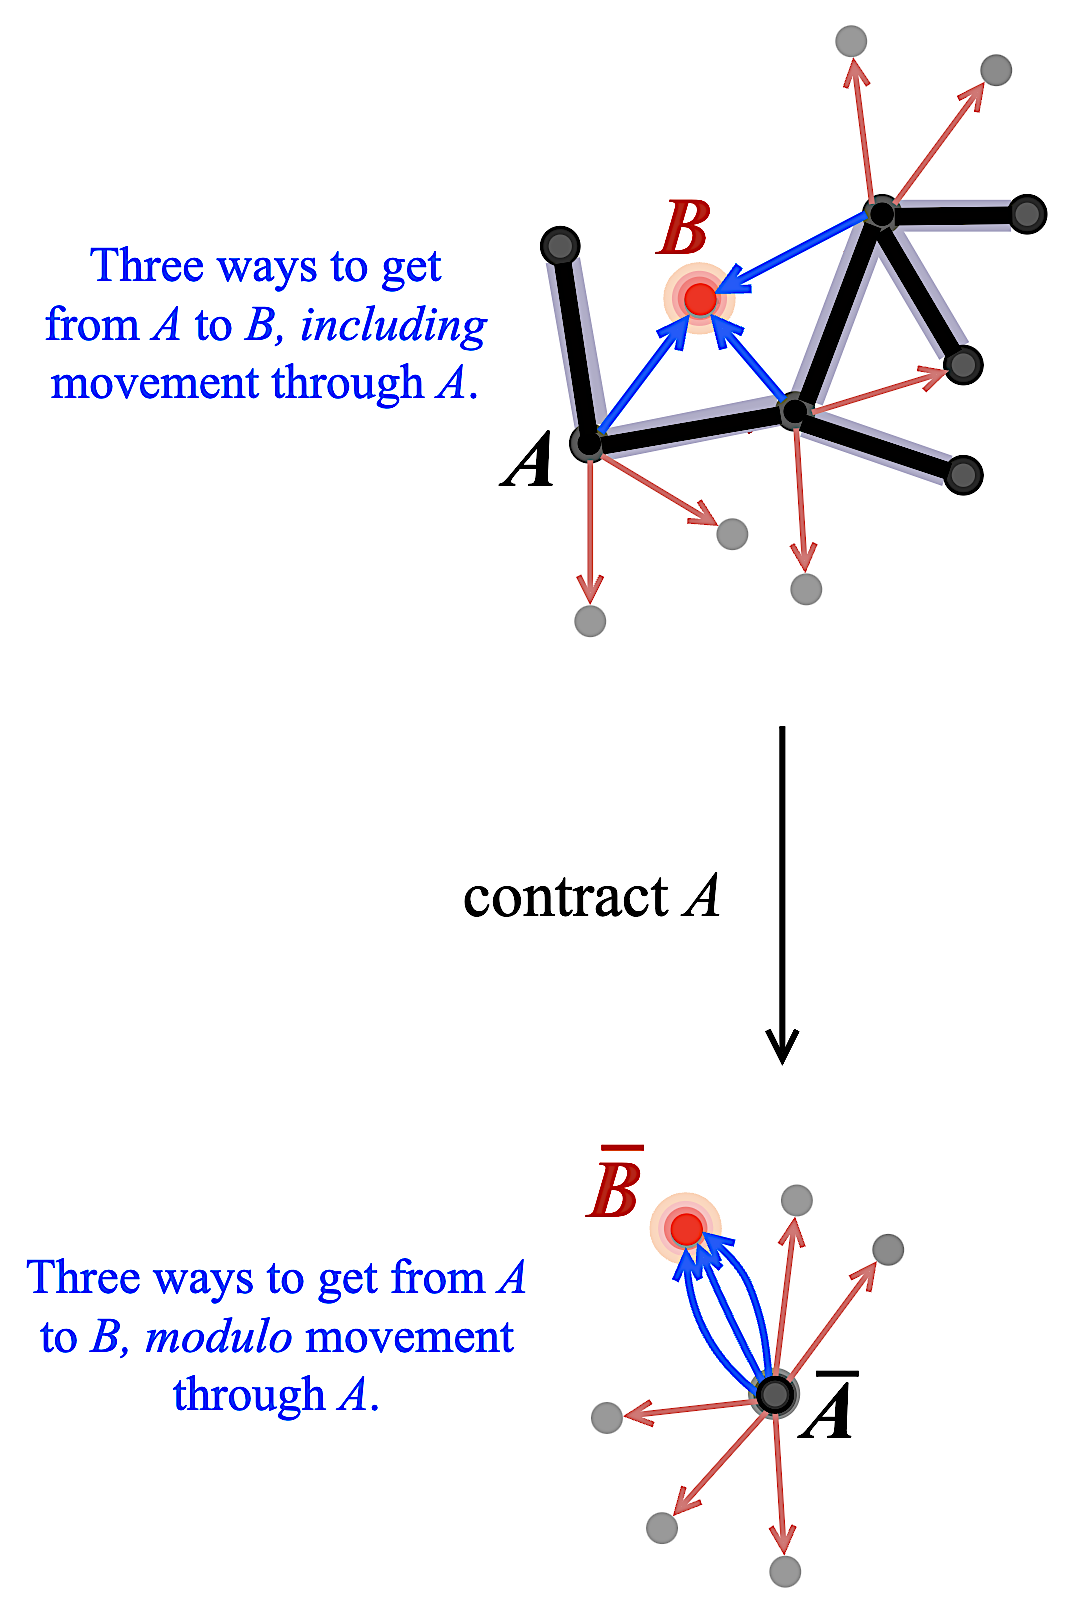
\includegraphics[scale=.3]{../../assets/images/mathematical_model/supertask.png}
    $$
    \vskip -.5cm
    \caption{Abstract supertasks as quotient states. A contracted graph cell may not name a familiar physical subtask, but it is meaningful operationally because it gathers concrete states with shared outgoing movement information. From the agent's perspective, choosing the coset is choosing a coarse address for many executable refinements.}
\end{figure}

\end{remark}

\end{subsection}

\end{section}

%\vskip .5cm

\begin{section}{Problem agnostic, hiearchical structure in RL}

\begin{subsection}{Dynamic state-space graph}

To each history $\gamma\in\bold{Path}(H)$ we associate two auxiliary, sequences of nested graphs and decorations.

\begin{definition}[{\bf Explored subgraph and viewed subgraph}]
\normalfont
Given a path $\gamma\in\bold{Path}(H)$, which is to say, a history
\begin{equation}\label{eq: gamma history}
\gamma=\left(s_{0}\xrightarrow{\ \alpha_{1}\ }s_{1}\xrightarrow{\ \alpha_{2}\ }\cdots\xrightarrow{\alpha_{k-1}}s_{k-1}\xrightarrow{\ \alpha_{k}\ }s_{k}\right)\quad\text{in}\quad H,
\end{equation}
for each integer time step $0\le t\le k$, we define the associated {\em visited subgraph at time $t$}, denoted $H^{0}_{t}$, to be the subgraph of $H$ formed by all states and actions visited by $\gamma$ up to and including time step $t$:
$$
H^{0}_{t}\;:=\;\gamma\left(s_{0}\xrightarrow{\ \alpha_{1}\ }s_{1}\xrightarrow{\ \alpha_{2}\ }\cdots\xrightarrow{\ \alpha_{t}\ }s_{t}\right)\;\text{as s subgraph of}\;H.
$$

Likewise, we define the associated {\em viewed subgraph at time $t$}, denoted $G^{0}_{t}$, to be the subgraph of $H$ formed by the union of the visited subgraph $H^{0}_{t}$ at times step $t$ and all outgoing $1$-hop neighborhoods $N^{\text{out}\!}_{1}(s)$ in $H$ at nodes in $H^{0}_{t}$ at time step $t$:
$$
G^{0}_{t}
\;:=\;
H^{0}_{t}\;\cup\bigcup_{s\in \mathcal{S}^{0}_{t}}
\!\!N^{\text{out}\!}_{1}(s)
$$
We let $\mathcal{S}^{0}_{t}$ and $\mathcal{A}^{0}_{t}$ denote the states and actions in $G^{0}_{t}$, i.e., the nodes and edges of $G^{0}_{t}$, respectively.
\end{definition}

\begin{remark}
\normalfont
By construction, we have chains of graph inclusions
$$
(\ \!{\color{black} s_0}\ \!)=H^{0}_{0}\;\subset\;(\ \!{\color{black} s_0\xrightarrow{\ \alpha_{1}\ }s_1}\ \!)=H^{0}_{1}
\;\subset\; H^{0}_{2}
\;\subset\; \cdots
\;\subset\; H^{0}_{k}.
$$
and
$$
\scalebox{.9}{$
\left(\ \ 
{\color{red}
\begin{xy}
(0,0)*+{{\color{black} s_0 }}="s0";
(15,0)*+{ s_{01}=s_{1}\!\!\!\!\!\!\!\!\!\!\!\!\!\!\!\!\!}="s1";
(9,12)*+{s_{02}}="s02";
(-9,12)*+{s_{03}}="s03";
(-15,0)*+{s_{04}}="s04";
(-6,-6)*+{\pmb{\ddots}}="sd1";
(9,-11)*+{s_{0,d_{0}}\!\!\!\!\!}="sd";
{\ar@{->} "s0"; "s1"};
{\ar@{->} "s0"; "s02"};
{\ar@{->} "s0"; "s03"};
{\ar@{->} "s0"; "s04"};
{\ar@{->} "s0"; "sd"};
\end{xy}
}
\ \ \ \ \ \ \ \ \ 
\right)
=G^{0}_{0}
\quad\subset\quad
\left(\ \ 
{\color{red}
\begin{xy}
(0,0)*+{{\color{black} s_0 }}="s0";
(17,0)*+{{\color{black} s_1 }}="s1";
(9,12)*+{s_{02}}="s02";
(-9,12)*+{s_{03}}="s03";
(-15,0)*+{s_{04}}="s04";
(-6,-6)*+{\pmb{\ddots}}="sd1";
(9,-11)*+{s_{0,d_{0}}\!\!\!\!\!}="sd";
{\ar@[black]^{{\color{black} \alpha_{1}}} "s0"; "s1"};
{\ar@{->} "s0"; "s02"};
{\ar@{->} "s0"; "s03"};
{\ar@{->} "s0"; "s04"};
{\ar@{->} "s0"; "sd"};
(30,0)*+{s_{11}=s_{2}\!\!\!\!\!\!\!\!\!\!\!\!\!\!\!\!\!\!\!\!\!\!}="s2";
(26,12)*+{s_{21}}="s12";
(26,-11)*+{s_{0,d_{1}}\!\!\!\!\!}="s1d";
{\ar@{->} "s1"; "s12"};
{\ar@{->} "s1"; "s02"};
{\ar@{->} "s1"; "s2"};
{\ar@{->} "s1"; "s1d"};
(13,-5)*+{\pmb{\ddots}};
\end{xy}
}
\ \ \ \ \ \ \ \ \ \ \ \ 
\right)
=G^{0}_{1}
\quad\subset\quad\cdots$}
$$
\end{remark}

\begin{definition}[{\bf Decorated viewed subgraph}]
\normalfont
Given a history as in \eqref{eq: gamma history}, we decorate each node $s$ of $G^{0}_{t}$, at each time step $t$, with its set of outgoing edges $\mathcal{A}_{H}(s)$ {\em inside} our ambient, hidden state/action-graph $H$.
\end{definition}

\begin{remark}
\normalfont
Note that if our state/action-graph $H$ has bounded degree, for instance if we know there are a finite and globally bounded number of degree of freedom to our problem at any given state, then decorating $G^{0}_{t}$ in this way requires a bounded number of adjacent $\mathcal{A}_{H}(s)$ checks, inducing a linear computational cost
$$
\Theta(t),\quad\text{where}\;t\;=\;\#\ \text{time steps}.
$$
The implementation should therefore treat the decoration as an incremental local update, not as a repeated scan of the whole explored graph. When a new state is reached, one queries the outgoing edge set at that state once and attaches the result to the node table. If the environment has bounded out-degree, this keeps the discovery cost linear in the number of visited states. The quadratic failure mode would come from rechecking outgoing neighborhoods at every endpoint of every previously discovered edge after each step.
\end{remark}



\end{subsection}

\begin{subsection}{Dynamic tower of quotient state-spaces}

We now contract all edges in $G^{0}_{t}$. However, we do to in a tiered manner, so that we contract edgers in stages, eventually exhausting all edges. 

We want to allow for both of the possibilities in Examples \ref{ex: actions match projections} and \ref{ex: point cloud}. In the case of Example \ref{ex: actions match projections}, the most obvious contraction schema is: (i) contract all $x$-axis actions, (ii) contract all $y$-axis actions, (iii) contract all $z$-axis actions. On a machine, this would mean labelling actions (\texttt{`x`}, ``$y$,'' or ``$z$'') and contracting according to label. In the case of Example \ref{ex: point cloud}, the randomness of the edges in $3$-space, and the randomness of out-degree from node to node, makes it difficult to contract them in any systematic way. A more natural strategy in this case is to sample $1/3$ of the outgoing, not yet sampled edges at each node in the original graph, and collapse them all to get next tier.

Although these two contraction schemas are very different, they have the same procedural outline, which we formalize as a ``contraction schema''

\begin{definition}
{\bf Contraction schemas.}
\normalfont
A {\em contraction schema} on a graph $G=\!\!\begin{xy}
(0,0)*+{\mathcal{A}}="1";
(12,0)*+{\mathcal{S}}="2";
{\ar@<2pt> "1"; "2"};
{\ar@<-2pt> "1"; "2"};
\end{xy}$ is any explicit or implicit ordered partition of its edge set
$
\mathcal{A}
=
\Sigma^1 \sqcup \Sigma^2 \sqcup \cdots \sqcup \Sigma^d,
$
such that we can retrieve each set $\Sigma^{i}$, one after the other.
\end{definition}

\begin{ermark}
{\bf Realization in code.}
\normalfont
On a machine, the contraction schema can take the form of a procedure that i.i.d. uniformly samples some fraction of the edges in the outgoing edge set at each node in $G$, waits for associated contraction subroutine to complete, and then samples same fraction from remaining arrows, contracting recursively in this way until the graph is completely contracted.
\end{ermark}

\begin{ermark}
{\bf Quotient tower construction: {\em Mathematical model}.}
\normalfont 
Figure~\ref{fig: dynamic tower} should be read as a top-to-bottom quotient process on the right-hand side. At the top, the hidden state/action-space has been dynamically mapped to the discovered graph $G_t^0=G_t$, with the current state $s_t^0=s_t$ and a marked family of edges to contract. The next diagram down is the first quotient $G_t^1$, obtained after carrying out the first contraction stage; below that is $G_t^2$, the second quotient. Thus the vertical direction in the figure is not refinement upward from a base graph, but successive contraction downward from the discovered graph to coarser quotient graphs.
\begin{figure}[!h]
	\vskip -.2cm
    $$
    \!\!\!\!
    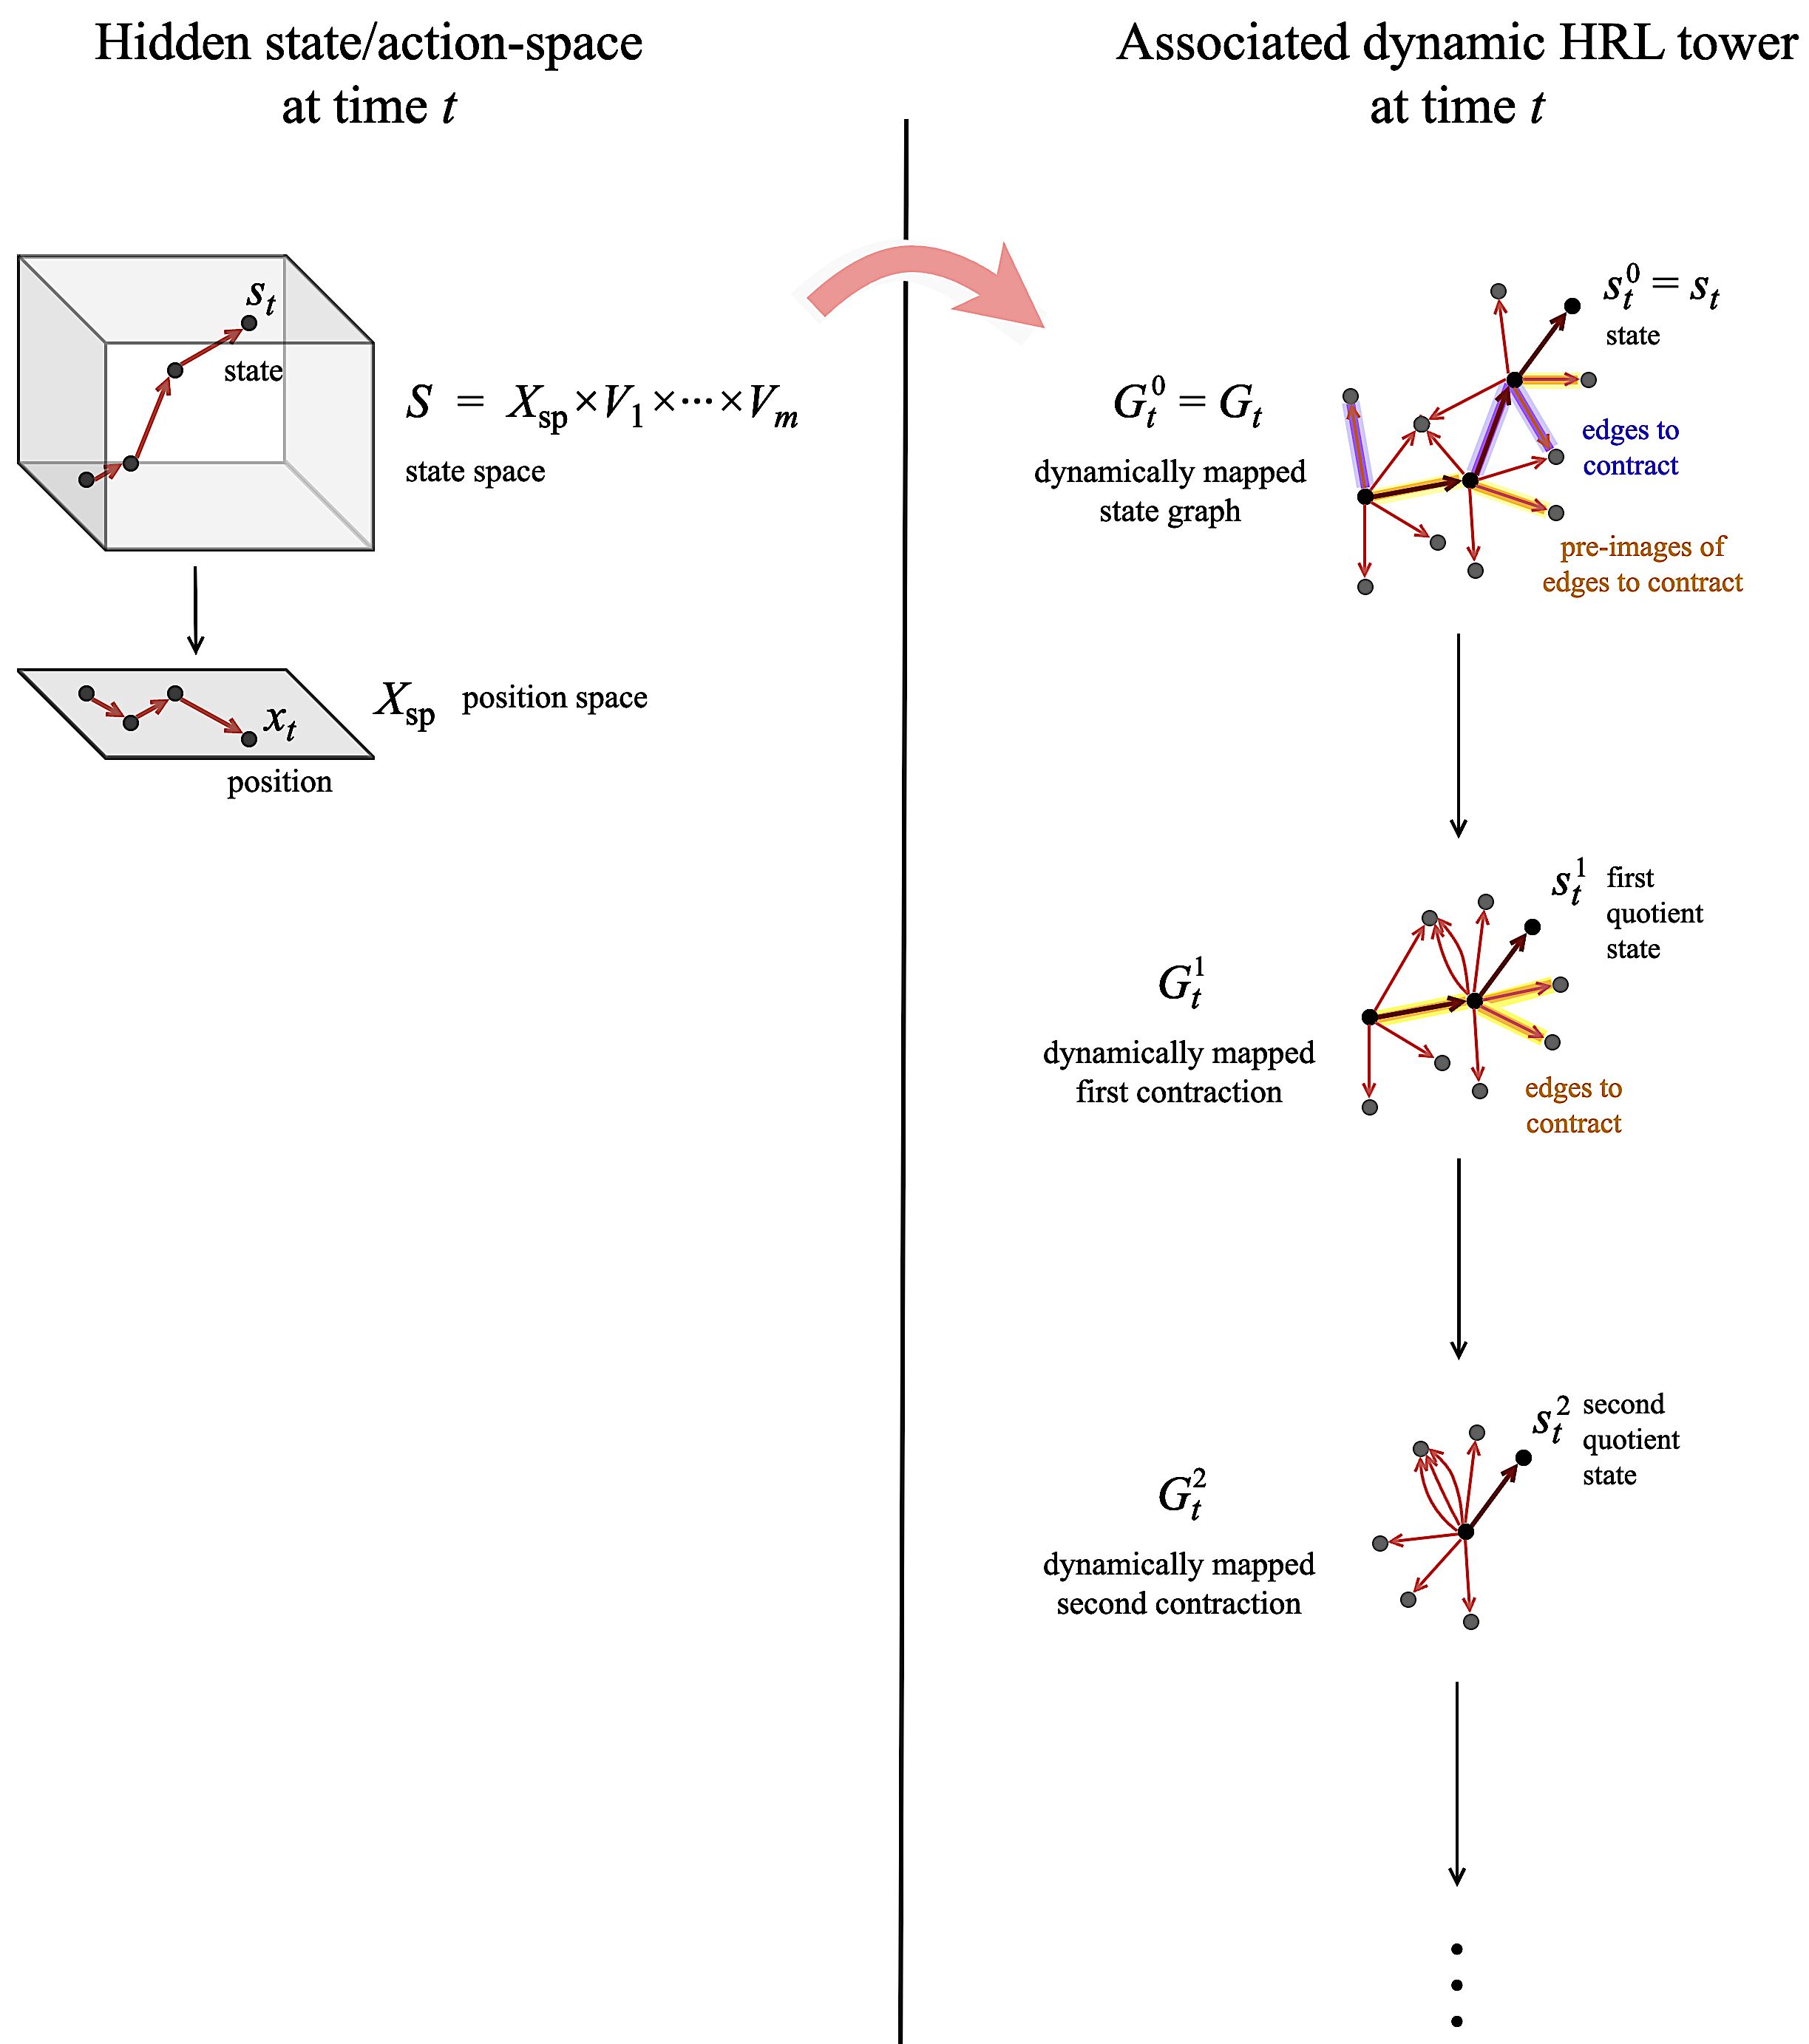
\includegraphics[scale=.7]{../../assets/images/mathematical_model/dynamic_tower.png}
    $$
    \vskip -.5cm
    \caption{Dynamic HRL tower associated to the hidden state/action-space at time $t$. The discovered graph $G_t^0=G_t$ appears at the top of the tower, and successive downward maps contract selected base-tier edges to produce $G_t^1,G_t^2,\ldots$, with the current state tracked through the corresponding quotient states $s_t^0,s_t^1,s_t^2,\ldots$.}
    \label{fig: dynamic tower}
\end{figure}

\end{ermark}

\begin{ermark}
{\bf Quotient tower construction: {\em Machine description}.}
\normalfont
In our mathematical model, we describe a graph $G$ as pairs of maps $\text{src},\text{tgt}:\mathcal{A}\longrightarrow\mathcal{S}$. Encoding this literal structure, in RAM, would amount to some sort of full adjacency graph encoding. 

Because primitive actions in state/action graphs tend to map to a relatively {\em very} small number of ``adjacent'' states, these graphs are extremely sparse. We encoded them sparsely, as a node set given by the state space $\mathcal{S}$ and, for each state $s\in\mathcal{S}$, a pointer to the outgoing edge set $\text{Out}(s):=\mathcal{A}(s)$.

We implement the quotient-tower in RAM by maintaining a nested system of labeled partitions of the base state set and base edge set under successive coarsening operations. This places the method near the classical partition-based data-structural viewpoint in algorithms \cite{PaigeTarjan1987} and \cite{HabibPaulViennot1999}. That said, the construction we now describe is not a {\em partion refinement algorithm} in the usual sense. Because the operative updates here encode graph edge contractions, they take the form of {\em coarsenings} of coupled state and action coset partitions. The tower is best understood as a coupled nested partition system adapted to contraction-driven quotient formation.

The base graph in memory already presents a node table together with an outgoing-edge table, and quotient construction begins by adjoining a state-partition table to this existing graph memory: we define the initial, {\em tier-}$0$ {\em state partition} to be the set of singletons, and we define its  associated {\em tier-}$0$ {\em action partition} to be the set of outgoing edge sets 
$$
\Pi_0^{\mathcal S}:=\bigl\{\{s\}\mid s\in\mathcal{S}_t^0\bigr\}
\qquad\text{and}\qquad
\Pi_0^{\mathcal A}:=\bigl\{\text{Out}(s)\mid s\in\mathcal{S}_t^0\bigr\},
$$
Note that each of the cells of $\Pi_0^{\mathcal A}$ is naturally associated to exactly one of the cells of $\Pi_0^{\mathcal S}$, namely its source state. In this way, me have a natural map
$$
\mathcal{A}^{0}_{t}\longrightarrow\Pi_0^{\mathcal S}
$$
that functions like ``a tangent bundle over state space,'' where the fiber over $\{s\}$ is $\text{Out}(s)$. Likewise, we have a map
$$
\Pi_0^{\mathcal S}\longrightarrow\Pi_0^{\mathcal A}
$$
that functions like the ``sheaf of tangent spaces over state space'' by  initializing a pointer at each tier-$0$ state partition cell $[s]_{0}:=\{s\}\in\Pi_0^{\mathcal S}$ that points to the cell $\text{Out}(s)$.

Inductively, suppose the tier-$(i-1)$ state and action partition tables have already been created. The $i$th tier is produced by opening fresh tier-$i$ tables initialized from tier $i-1$, then processing every arrow in the contraction block $\Sigma^i$. For an arrow $a\xrightarrow{\ e\ }b$, we look up the tier-$(i-1)$ cells containing $a$ and $b$. If they are distinct, we create a new tier-$i$ state-cell representing their union and a new tier-$i$ outgoing action-cell collection representing the union of their outgoing data, after discarding actions that have become loops inside the merged cell. The affected base nodes receive tier-$i$ pointers to the new cell. Repeating this through the block yields $G_t^i$.

The inductive step from tier $i-1$ to tier $i$ is driven by the $i$th block $\Sigma^i$ of the base-edge contraction schema. For each edge $a\xrightarrow{\ e\ }b$ in this block, let $C_a$ and $C_b$ be the current state-cells containing its endpoints. If $C_a\neq C_b$, we create a new tier-$i$ state-cell $C_{ab}$ by coalescing $C_a$ and $C_b$, and we create the corresponding tier-$i$ action-cell data by coalescing their outgoing action-cell collections. Pointers from all nodes in $C_a\cup C_b$ are then initiated to $C_{ab}$, and $C_{ab}$ is pointed to its merged outgoing-action collection. Repeating this for all arrows in $\Sigma^i$ gives the next partition layer.

We apply the graph quotienting procedure to this data structure as a sequence of successive parallel coarsening of two coupled partition systems. Assume, by finite induction, that at tier $i$ the \emph{state-side partition table} is a finite labeled partition
\[
\Pi_i^{\mathcal S}=\{C_{i,\lambda}^{\mathcal S}\}_{\lambda\in I_i^{\mathcal S}}
\quad\text{of}\quad\mathcal{S}_t^0,
\]
and the \emph{action-side partition table} is a finite labeled partition
\[
\Pi_i^{\mathcal A}=\{C_{i,\mu}^{\mathcal A}\}_{\mu\in I_i^{\mathcal A}}
\quad\text{of}\quad\mathcal{A}_t^0
\]
such that each cell $C_{i,\mu}^{\mathcal A}$ lies over a single state partition cell $C_{i,\lambda}^{\mathcal S}$, in the sense that there exists a state partition cell $C_{i,\lambda}^{\mathcal S}$ in $\Pi_i^{\mathcal S}$ such that for all actions $\alpha\in C_{i,\mu}^{\mathcal A}$, we have
	$$
	\text{src}(\alpha)\in C_{i,\lambda}^{\mathcal S}
	$$
This ensures that at tier-$i$, we have a tangent bundle-like map 
$$
\mathcal{A}^{0}_{t}\longrightarrow\Pi_i^{\mathcal S}
$$
Each node in our original graph, $s\in\mathcal{S}_t^0$, carries a pointer to its current state-cell $[s]_i\in\Pi_i^{\mathcal S}$, and that state-cell carries a pointer to its current outgoing action-cell collection $\mathrm{Out}_i([s]_i)$. Thus we also have a tangent sheaf-like map
$$
\Pi_i^{\mathcal S}\longrightarrow\Pi_i^{\mathcal A}
$$

\begin{figure}[!h]
    \vskip -.5cm
    $$
    \!\!\!\!\!\!\!\!\!\!
    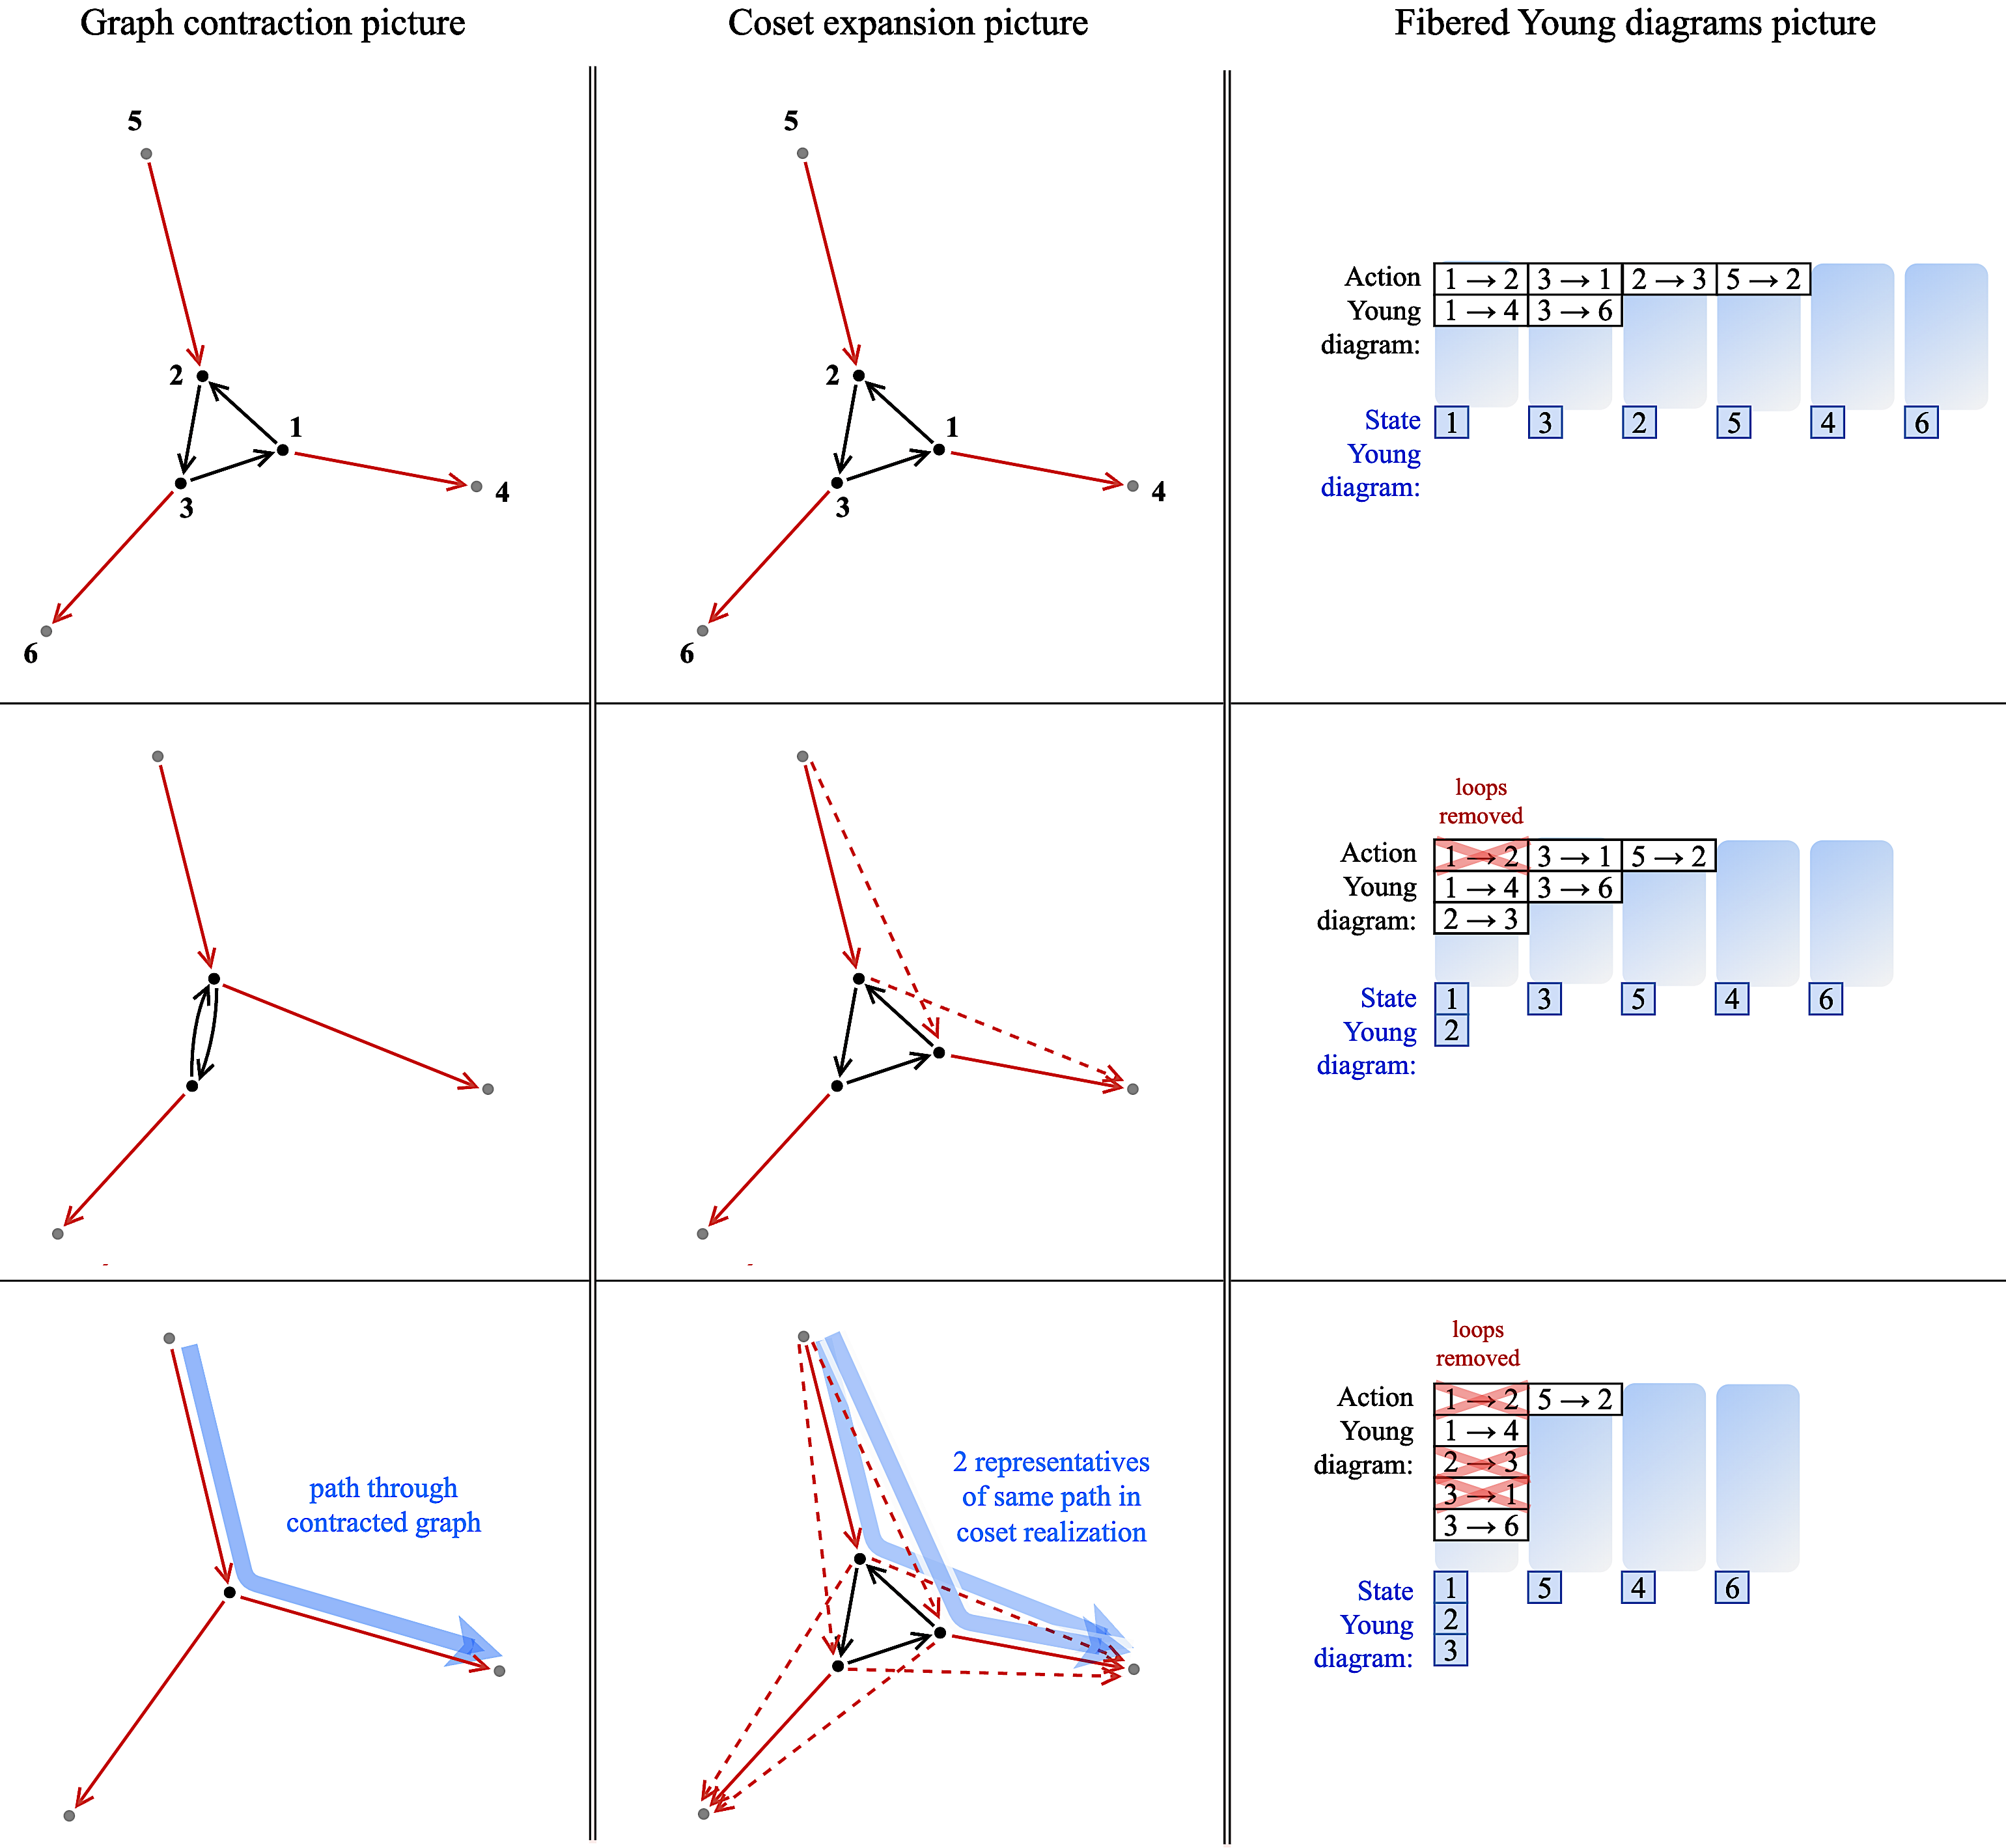
\includegraphics[scale=.65]{../../assets/images/mathematical_model/3ways.png}
    $$
    \vskip -.5cm
    \caption{Successive contraction of $3$ edges in a graph: (Left) Graph-contraction picture. (Middle) Coset-expanding picture. (Right) Nested, fibered partitions (Young tableaux) structures in RAM encoding the contractions in a light weight, easy to traverse manner.}
    \label{fig:three_pictures_tower}
\end{figure}

Figure~\ref{fig:three_pictures_tower} shows the same quotient-tower construction from three compatible points of view. On the left is the graph-contraction picture: selected arrows identify states, internal arrows of a merged cell become loops and are discarded, and the remaining red arrows become outgoing quotient actions. In the middle is the coset-expansion picture: a quotient state is not a new physical state, but a coset of base states, and each representative of the coset inherits the outgoing-action information available from the other representatives. Thus one coarse path through the contracted graph can have several base-level realizations. On the right is the data-structure picture: the tower is stored as nested state Young diagrams together with nested action Young diagrams, with action cells fibered over state cells by outgoing-incidence pointers. The same construction is therefore simultaneously a graph quotient, an operational sharing of outgoing information across cosets, and a coupled coarsening of state/action partition tables in memory.

Abstractly, each partition layer can be drawn like a labeled Young diagram \cite{YoungTab}. The cells are the blocks o the diagram, and the entries in a cell are the base states or base actions that have been identified at that tier. The tower is then a nested sequence of such labeled diagrams, with cells in one tier sitting inside larger cells in the next. We introduce a bit of extra structure action diagram is fibered over the state diagram by outgoing-incidence pointers: each state-cell carries a decoration naming the action-cell collection available from that coset.

The tower is nested because these partitions coarsen with $i$. Each state-cell at tier $i$ lies inside a unique state-cell at tier $i+1$, and likewise each action-cell at tier $i$ lies inside a unique action-cell at tier $i+1$. Thus the actual tower object is best understood as: (i) the fixed discovered base graph $G_t^0$, (ii) a nested tower of labeled state partitions $\Pi_0^{\mathcal S},\Pi_1^{\mathcal S},\dots$, (iii) a nested tower of labeled action partitions $\Pi_0^{\mathcal A},\Pi_1^{\mathcal A},\dots$, (iv) and, at each tier, the outgoing-incidence pointers from state-cells to action-cells.

The pseudocode below should be read in these terms.

\begin{figure}[!h]
\begin{algorithm}[H]
\caption{Successive Quotients via Nested State/Action Coset Partitions}
\label{alg: successive_quotients_nested_cosets}
\begin{algorithmic}[1]

\Require
Current discovered base graph $G_t^0=(\mathcal{S}_t^0,\;\mathcal{A}_t^0)$,
a current base state $s_t\in \mathcal{S}_t^0$, and an explicit or implicit ordered partition of the base-tier edge set
$
\mathcal{A}_t^0
=
\Sigma_0^1 \sqcup \Sigma_0^2 \sqcup \cdots \sqcup \Sigma_0^d.
$
%Regard the discovered graph in memory as: 1. a node table on $\mathcal{S}_t^0$, together with 2. the outgoing-edge table $\mathcal{A}_t^0(s)$ indexed by source node $s$.

\Ensure
A tower $G_t^0 \twoheadrightarrow G_t^1 \twoheadrightarrow \cdots \twoheadrightarrow G_t^N$ in the form of nested state/action coset partitions decorating $G_t^0$.

\Statex

\Function{BuildTower}{$G_t^0,s_t$}

%\Statex

    \Statex {\bf \!\!\!\!\!\!\!\!\!Initialization:}

    \State Initialize the tier-$0$ state-partition table by singletons:
    $
    [s]_0 \gets \{s\}
    $
    for each $s\in\mathcal{S}_t^0$.

    \For{$s\in\mathcal{S}_t^0$}
    \State Initialize the tier-$0$ action-side partition table by the outgoing edges:
    $
    \mathrm{Out}_0([s]_0)\gets \mathcal{A}_t^0(s)
    $
        \State Initiate a tier-$0$ pointer from $s$ to its state-cell $[s]_0$.
        \State Initiate a tier-$0$ pointer from $[s]_0$ to its outgoing-action cell collection $\mathrm{Out}_0([s]_0)$.
    \EndFor

    \State $G_t^0$ in memory $\gets$ node table on $\mathcal{S}_t^0$ decorated by the tier-$0$ state and action partition pointers.

%    \Statex
    \Statex {\bf \!\!\!\!\!\!\!\!\!Inductive step:}
    \State $i \gets 1$
    \While{$i \le d$}

        \State Copy previous partition tables forward as initial tier-$i$ tables:
        $
        \Pi_i^{\mathcal S}\gets \Pi_{i-1}^{\mathcal S},
        \;
        \Pi_i^{\mathcal A}\gets \Pi_{i-1}^{\mathcal A}
        $

        \For{$a\xrightarrow{\ e\ }b \in \Sigma_0^i$}
            \State Let $C_a\in\Pi_{i-1}^{\mathcal S}$ be the tier-$(i-1)$ state-cell containing $a$.
            \State Let $C_b\in\Pi_{i-1}^{\mathcal S}$ be the tier-$(i-1)$ state-cell containing $b$.

            \If{$C_a\neq C_b$}
                \State Coalesce state data into new tier-$i$ state cell:
                $
                C_{ab}\gets \mathrm{MergeStateCells}(C_a,C_b)
                $

                \State  Associate tier-$(i-1)$ action cells: $D_a:=\mathrm{Out}_{i-1}(C_a),\;D_b:=\mathrm{Out}_{i-1}(C_b)$

                \State Coalesce action data into new tier-$i$ action cell:
                $
                D_{ab}\gets \mathrm{MergeActionCells}(D_a,D_b)
                $
                
                \State Remove from $D_{ab}$ all actions whose source and target both lie in $C_{ab}$, recording their contribution according to the chosen stutter convention.

	       \For{node in $C_a\cup C_b$}
                \State Initiate new tier-$i$ pointer to new tier-$i$ state-cell $C_{ab}$.

                \State Initiate new tier-$i$ pointer from $C_{ab}$ to new tier-$i$ action cell $D_{ab}$.
                \EndFor
            \EndIf
        \EndFor

        \For{$s\in\mathcal{S}_t^0$}
            \State Initiate new pointer from node $s$  to its tier-$i$ state-cell $[s]_i\in\Pi_i^{\mathcal S}$
            \State Initiate new pointer from node $s$  to its action cell collection $\mathrm{Out}_i([s]_i)\subseteq\Pi_i^{\mathcal A}$
        \EndFor

        \State $G_t^i$ in memory $\gets$ same node table on $\mathcal{S}_t^0$, but with these pointers to $\Pi_i^{\mathcal S}$, $\Pi_i^{\mathcal A}$

        \State $i \gets i+1$

    \EndWhile

    \State \Return $\bigl(
    G_t^0,G_t^1,\dots,G_t^N
    \bigr)$
\EndFunction

\end{algorithmic}
\end{algorithm}
    \label{fig: algorithm 1}
\end{figure}

\end{ermark}

\begin{remark}
{\bf Traversing the tower}
\normalfont
An RL agent can traverse this representation of the graph just as well as the adjacency representation, but the sparse representation is easier on memory.

The key point is that traversal in the quotient tower is not the same as taking an edge whose source is literally the current base node. At tier $i$, the agent is located at a state-cell $[s]_i$, and that cell carries outgoing-action information pooled from all of its representatives. The agent may therefore choose an abstract outgoing action whose concrete representative starts at some other node in the same coset. Execution then requires a lift/refinement step: move within the coset, or select a representative path, so that the abstract action becomes executable in the base graph. This is exactly why the coset must carry unified outgoing-action data. The tower lets the agent jump through quotient addresses first and resolve concrete source compatibility only when lifting back down.
\end{remark}

\begin{run_analysis}
{\bf Runtime analysis of Algorithm~\ref{alg: successive_quotients_nested_cosets}}
\normalfont
We now analyze the cost of Algorithm~\ref{alg: successive_quotients_nested_cosets} as written.

Define
$
n_t:=|\mathcal{S}_t^0|$,
$
m_t:=|\mathcal{A}_t^0|$, and recall that $d$ is the number of blocks in our implicit contracting partition
$\mathcal{A}_t^0
=
\Sigma_0^1 \sqcup \Sigma_0^2 \sqcup \cdots \sqcup \Sigma_0^d
$.
It's important here that $d$ is like a characteristic constant of the problem that can be interpreted as the dimension of the problem's underlying state space, so that $|\mathcal{S}_t^0|\sim \ell^{d}$, where $\ell$ is some variable representing ``the expected length of one dimension of the problem.'' In other words, we should think of $d$ as being
\begin{equation}\label{eq: approx log}
d\;\sim\;\text{log}_{\ell}\,|\mathcal{S}_t^0|\;=\;\text{log}_{\ell}\,n_{t}
\end{equation}
...There's also a natural argument that the expect nature of the sparsity in state/action graphs gives us the following expected value of $m_{t}$ is
$$
m_{t}
\;\sim\;
n_{t}\,d
\;\sim\;
n_{t}\,\text{log}_{\ell}\,n_{t}
$$
Write
$
m_i:=|\Sigma_0^i|$, so that $\sum_{i=1}^d m_i=m_t.
$
Thus every base-tier edge is processed exactly once by the contraction schedule.

\paragraph{Initialization cost.}
The initialization phase consists of:
\begin{enumerate}
    \item creating the singleton state-partition cells $[s]_0$ for all $s\in\mathcal{S}_t^0$,
    \item reading off the outgoing-edge buckets $\mathcal{A}_t^0(s)$,
    \item and initiating the tier-$0$ node-to-state and state-to-action pointers.
\end{enumerate}
The singleton initialization costs $O(n_t)$, while reading the outgoing-edge table costs $O(m_t)$ if the adjacency structure is already present in memory, or $O(n_t+m_t)$ if it must be traversed by source. Hence the full initialization cost is
\[
T_{\mathrm{init}}=O(n_t+m_t).
\]

\paragraph{Per-tier cost.}
Fix a tier index $i\in\{1,\dots,d\}$. As written, the tier-$i$ work has three parts.

First, the algorithm copies the previous partition tables forward and later re-initiates the node pointers for all states. The explicit final loop
\[
\texttt{for }s\in\mathcal{S}_t^0
\]
already contributes $O(n_t)$ work per tier, regardless of how many contractions actually occur in $\Sigma_0^i$.

Second, the algorithm processes the edge block $\Sigma_0^i$. For each
\[
a\xrightarrow{\ e\ }b\in\Sigma_0^i
\]
it performs:
\begin{enumerate}
    \item two state-cell lookups,
    \item one state-cell coalescence if the cells differ,
    \item one action-cell lookup on each side,
    \item one action-cell coalescence,
    \item and pointer initiation for all nodes in the merged state-cell.
\end{enumerate}
If we denote by
$
U_i^{\mathcal S}
$
the total cost of all state-cell coalescences and their induced node-pointer updates at tier $i$, and by
$
U_i^{\mathcal A}
$
the total cost of all action-cell coalescences at tier $i$, then the edge-processing loop contributes
\[
O(m_i + U_i^{\mathcal S}+U_i^{\mathcal A}).
\]

Third, the algorithm stores the resulting tier-$i$ decorations back into the in-memory graph view, which is again accounted for by the explicit node loop and therefore contributes no asymptotically new term beyond $O(n_t)$.

Accordingly, the total cost of tier $i$ is
\[
T_i = O\bigl(n_t + m_i + U_i^{\mathcal S}+U_i^{\mathcal A}\bigr).
\]

\paragraph{Total runtime.}
Summing over all tiers gives
\[
T_{\mathrm{BuildTower}}
=
T_{\mathrm{init}} + \sum_{i=1}^d T_i
=
O(n_t+m_t)
+
\sum_{i=1}^d O\bigl(n_t + m_i + U_i^{\mathcal S}+U_i^{\mathcal A}\bigr).
\]
Using $\sum_{i=1}^d m_i=m_t$, this simplifies to
\[
T_{\mathrm{BuildTower}}
=
O\!\left(
d\,n_t + m_t + \sum_{i=1}^d U_i^{\mathcal S} + \sum_{i=1}^d U_i^{\mathcal A}
\right).
\]
This is the correct general bound for the pseudocode as stated.

By \eqref{eq: approx log}, we can expect this to be
\[
T_{\mathrm{BuildTower}}
=
O\!\left(
n_t\,\text{log}_{\ell}\,n_{t} + 
\!\!\!\!\!
\underset{\text{by sparsity}}{\underset{\text{controlled}}{\underbrace{m_t}}}
 + \sum_{i=1}^d U_i^{\mathcal S} + \sum_{i=1}^d U_i^{\mathcal A}
\right).
\]
[It's an important point here that almost all real life control problems are sparse, since states can only move to nearby states...]

\paragraph{What depends on the coalescence implementation.}
The terms $
U_i^{\mathcal S}$ and 
$U_i^{\mathcal A}$ depend entirely on how the partition tables are implemented.

\begin{itemize}
    \item If state-cell and action-cell coalescence are implemented naively by explicit member copying and repeated pointer rewriting, then these terms can be large, and in the worst case one can obtain quadratic behavior inside a tier.

    \item If cell coalescence is implemented by a standard union-by-size or union-by-rank discipline, then within a fixed tier each base element changes its canonical representative only logarithmically many times. In that case, one obtains the tierwise bounds
    \[
    U_i^{\mathcal S}=O(n_t\log n_t),
    \qquad
    U_i^{\mathcal A}=O(m_t\log m_t),
    \]
    and therefore
    \[
    T_i
    =
    O\bigl(n_t + m_i + n_t\log n_t + m_t\log m_t\bigr).
    \]
    Summing over $i$ then yields the worst-case bound
    \[
    T_{\mathrm{BuildTower}}
    =
    O\bigl(
    d\,n_t\log n_t + d\,m_t\log m_t + d\,n_t + m_t
    \bigr).
    \]
\end{itemize}

\paragraph{Interpretation of the bound.}
This worst-case bound should not be misread as the actual expected runtime burden in the online setting. Two structural facts matter.

First, the ordered partition
\[
\mathcal{A}_t^0
=
\Sigma_0^1 \sqcup \Sigma_0^2 \sqcup \cdots \sqcup \Sigma_0^d
\]
ensures that each base-tier edge participates in the contraction schedule exactly once. Thus the algorithm is not repeatedly rescanning the full edge set at every tier.

Second, and more importantly for the runtime story of the package, Algorithm~\ref{alg: successive_quotients_nested_cosets} is the \emph{full-build} description. In the actual online setting, one does not repeatedly rebuild the whole tower from scratch at each time step $t$. Instead, one uses the incremental update algorithm: if a realized move produces no new exploration, then
\[
G_{t+1}^\bullet = G_t^\bullet;
\]
and if a realized move does produce new exploration, then only the newly discovered base-tier edges are propagated upward through the existing partition tables. The full-build bound above is therefore the correct static cost of the construction, but it substantially overstates the expected amortized online cost.

\paragraph{Space usage.}
As written, the algorithm stores:
\begin{enumerate}
    \item the base node table on $\mathcal{S}_t^0$,
    \item the base outgoing-edge table on $\mathcal{A}_t^0$,
    \item one state-partition layer per tier,
    \item one action-partition layer per tier,
    \item and node-to-state / state-to-action pointer decorations at each tier.
\end{enumerate}
Thus the explicit space usage is at least linear in the base graph size and linear in the number of tiers:
$
O(d\,n_t + d\,m_t)
$
up to implementation-dependent constants. With structural sharing between tiers, the effective memory burden can be much smaller, but the displayed bound is the correct straightforward bound for the pseudocode as written.

\paragraph{Conclusion.}
Algorithm~\ref{alg: successive_quotients_nested_cosets} is therefore best viewed as a clear \emph{static specification} of the quotient-tower construction. Its full-build runtime is governed by:
\[
O\!\left(
d\,n_t + m_t + \sum_{i=1}^d U_i^{\mathcal S} + \sum_{i=1}^d U_i^{\mathcal A}
\right),
\]
with the precise asymptotics determined by the partition-coalescence implementation. The online package runtime is lighter because the next algorithm replaces wholesale rebuilding by incremental propagation of only newly discovered base-tier edges.
\end{run_analysis}

\begin{ermark}

\begin{figure}[!h]
\begin{algorithm}[H]
\caption{Incremental Tower Update Along Exploration}
\label{alg: incremental_tower_update}
\begin{algorithmic}[1]

\Require
A current decorated tower
$
G_t^0 \twoheadrightarrow G_t^1 \twoheadrightarrow \cdots \twoheadrightarrow G_t^N
$
in memory, a realized move from $s_t$ to a genuinely new state $s_{t+1}$, with updated discovered base graph $G_{t+1}^0=(\mathcal{S}_{t+1}^0,\;\mathcal{A}_{t+1}^0)$.

\Ensure
An updated tower
$
G_{t+1}^0 \twoheadrightarrow G_{t+1}^1 \twoheadrightarrow \cdots \twoheadrightarrow G_{t+1}^{N'}
$
in the form of nested state/action coset partitions decorating $G_{t+1}^0$, together with tower morphisms
$
G_t^\bullet \longrightarrow G_{t+1}^\bullet.
$

\Statex

\Function{UpdateTower}{$G_t^\bullet,s_t,s_{t+1}$}

    \State $\Delta\mathcal{A}_{t+1}^0 \gets \mathcal{A}_{t+1}^0\setminus \mathcal{A}_t^0$
    \State $\Delta\mathcal{S}_{t+1}^0 \gets \mathcal{S}_{t+1}^0\setminus \mathcal{S}_t^0$

    \State Regard the updated discovered graph in memory as:
    1. the node table on $\mathcal{S}_{t+1}^0$, together with
    2. the outgoing-edge table $\mathcal{A}_{t+1}^0(s)$ indexed by source node $s$.

%    \Statex
    \Statex {\bf \!\!\!\!\!\!\!\!\!Initialization:}

    \For{$s\in\mathcal{S}_t^0$}
        \State Keep the existing tier-$0$ state pointer from $s$ to $[s]_0$.
        \State Replace the tier-$0$ action pointer at $[s]_0$ with new edge bucket
        $
        \mathrm{Out}_0([s]_0)\gets \mathcal{A}_{t+1}^0(s).
        $
    \EndFor

    \State Initialize a new singleton tier-$0$ state-cell for the new state:
    $
    [s_{t+1}]_0\gets \{s_{t+1}\}.
    $

    \State Initialize its tier-$0$ outgoing-action cell:
    $
    \mathrm{Out}_0([s_{t+1}]_0)\gets \mathcal{A}_{t+1}^0(s_{t+1}).
    $

    \State Initiate a tier-$0$ pointer from $s_{t+1}$ to $[s_{t+1}]_0$.
    \State Initiate a tier-$0$ pointer from $[s_{t+1}]_0$ to $\mathrm{Out}_0([s_{t+1}]_0)$.

    \State $G_{t+1}^0$ in memory $\gets$ node table on $\mathcal{S}_{t+1}^0$ wiht tier-$0$ state and action partition pointers.

    \State Determine partition
    $
    \Delta\Sigma_0^1,\Delta\Sigma_0^2,\dots,\Delta\Sigma_0^d
    $
    of the newly discovered edge set $\Delta\mathcal{A}_{t+1}^0$, where $\Delta\Sigma_0^i$ is the tier-$i$ contraction list contributed by the new vista.

%    \Statex
    \Statex {\bf \!\!\!\!\!\!\!\!\!Inductive step:}

    \State $i \gets 1$
    \While{$i \le d$}

        \State Initialize the tier-$i$ partition tables by carrying forward the tier-$(i-1)$ structure on all previously existing nodes and cells.

        \For{$a\xrightarrow{\ e\ }b \in \Delta\Sigma_0^i$}
            \State Let $C_a\in\Pi_{i-1}^{\mathcal S}$ be the tier-$(i-1)$ state-cell containing $a$.
            \State Let $C_b\in\Pi_{i-1}^{\mathcal S}$ be the tier-$(i-1)$ state-cell containing $b$.

            \If{$C_a\neq C_b$}
                \State Coalesce the state data into a new tier-$i$ state-cell:
                $
                C_{ab}\gets \mathrm{MergeStateCells}(C_a,C_b).
                $

                \State Define associated tier-$(i-1)$ action cells: $D_a:=\mathrm{Out}_{i-1}(C_a)$ and $D_b:=\mathrm{Out}_{i-1}(C_b)$

                \State Coalesce into a new tier-$i$ action cell:
                $
                D_{ab}\gets \mathrm{MergeActionCells}(D_a,D_b).
                $

                \State Remove from $D_{ab}$ all actions whose source and target both lie in $C_{ab}$, recording their contribution according to the chosen stutter convention.

                \For{node in $C_a\cup C_b$}
                    \State Initiate a tier-$i$ pointer from that node to the new tier-$i$ state-cell $C_{ab}$.
                \EndFor

                \State Initiate a tier-$i$ pointer from $C_{ab}$ to the new tier-$i$ outgoing action cell $D_{ab}$.
            \EndIf
        \EndFor

        \For{$s\in\mathcal{S}_{t+1}^0$}
            \If{$s$ received no new tier-$i$ state pointer during the preceding loop}
                \State Keep its inherited tier-$i$ state pointer from the carried-forward tier-$(i-1)$ structure.
            \EndIf

            \If{the tier-$i$ state-cell containing $s$ received no new outgoing pointer during the preceding loop}
                \State Keep its inherited tier-$i$ outgoing pointer from the carried-forward tier-$(i-1)$ structure.
            \EndIf
        \EndFor

        \State $G_{t+1}^i$ in memory $\gets$ the same node table on $\mathcal{S}_{t+1}^0$, now decorated by the tier-$i$ state-cell pointers and tier-$i$ outgoing-action pointers.

        \State Define the tier morphism
        $
        G_t^i \longrightarrow G_{t+1}^i
        $
        by sending each old tier-$i$ state-cell to the unique new tier-$i$ state-cell containing it, and similarly on the associated outgoing-action cells.

        \State $i \gets i+1$

    \EndWhile

    \State Let $N'$ be the largest tier index created by the above update.

    \State Assemble the tower morphism
    $
    G_t^\bullet \longrightarrow G_{t+1}^\bullet
    $
    from these tierwise maps.

    \State Update the active state pointer so that the current node is now $s_{t+1}$.

    \State \Return $\bigl(
    G_{t+1}^0,G_{t+1}^1,\dots,G_{t+1}^{N'}
    \bigr)$
\EndFunction

\end{algorithmic}
\end{algorithm}
    \label{fig: algorithm 2}
\end{figure}

\end{ermark}

\end{subsection}

\end{section}

%\vskip .5cm

\begin{section}{Path-volume and logarithmic speed-up.}

\begin{subsection}{Finite-horizon path-volume}

For a finite state/action graph $G$, let
$
\bold{Path}_{k}(G)
$
denote the set of length-$k$ histories in $G$, and let
$$
\bold{Path}_{\le K}(G)
:=
\bigsqcup_{k=0}^{K}\bold{Path}_{k}(G)
$$
denote the finite-horizon path space through horizon $K$.
Write
$$
N_k(G):=\bigl|\bold{Path}_{k}(G)\bigr|
\qquad\text{and}\qquad
N_{\le K}(G):=\sum_{k=0}^{K}N_k(G).
$$
If every state had exactly $d$ outgoing actions, and if every path were admissible, then $N_k(G)$ would grow like $d^k$, up to the number of allowed initial states. Real RL environments differ from this naive model because of invalid moves, termination rules, policy bias, hard constraints, symmetries, and reward irrelevance. The point of the following definition is to keep both pieces of information visible: the exponential branching model and the actual finite path count.

\begin{definition}[{\bf Path-volume series}]\label{def:path-volume-series}
\normalfont
Fix a reference branching number $d\ge 1$. The finite-horizon path-volume series of $G$ at horizon $K$ is
$$
\PVol_G(d;K)
:=
\sum_{k=0}^{K}c_kd^k,
$$
where
$$
c_k:=\frac{N_k(G)}{d^k}.
$$
Equivalently,
$$
\PVol_G(d;K)=N_{\le K}(G).
$$
The coefficients $c_k$ record the deviation between the naive $d^k$ branching model and the actual admissible path count.
\end{definition}

The notation is deliberately redundant. The expression $\sum c_kd^k$ remembers the path-space growth intuition, while the equality with $N_{\le K}(G)$ makes the quantity a finite combinatorial invariant.

\begin{definition}[{\bf Policy-effective path-volume}]\label{def:policy-effective-path-volume}
\normalfont
Let $\pi_\theta$ be a policy, and let
$
\mu_{\theta,k}\in \Delta(\bold{Path}_k(G))
$
be the distribution on length-$k$ histories induced by $\pi_\theta$, the environment transition rule, and the reward/termination mechanism. For a threshold $\varepsilon>0$, define the effective support at length $k$ by
$$
N_k^{\theta,\varepsilon}(G)
:=
\left|
\left\{
\gamma\in\bold{Path}_k(G)
\,:\,
\mu_{\theta,k}(\gamma)\ge\varepsilon
\right\}
\right|.
$$
The $\varepsilon$-effective path-volume is
$$
\PVol_G^{\theta,\varepsilon}(K)
:=
\sum_{k=0}^{K}N_k^{\theta,\varepsilon}(G).
$$
An entropy-based variant replaces support size by $\exp(H(\mu_{\theta,k}))$.
\end{definition}

The raw path-volume is a worst-case geometric object. The policy-effective path-volume is closer to a training diagnostic. Both matter: the first describes the ambient path-space burden, while the second measures the portion of that burden the current learner is actually sampling.

\begin{warning}[{\bf Finite horizon only}]
\normalfont
The informal expression
$
\sum_{k\ge0}d^k
$
is useful as a slogan for path-space explosion, but it is not a finite complexity invariant unless it is truncated or discounted. All statements below use a finite horizon $K$, or else an explicitly discounted variant.
\end{warning}

\end{subsection}

\begin{subsection}{Path addresses induced by the partition tower}

Algorithm~\ref{alg: successive_quotients_nested_cosets} does not rebuild an independent quotient graph from scratch at each tier. It keeps the discovered base graph
$
G_t^0=(\mathcal{S}_t^0,\mathcal{A}_t^0)
$
in memory, and constructs two nested partition systems over it:
$$
\Pi_0^{\mathcal S},\Pi_1^{\mathcal S},\ldots,\Pi_N^{\mathcal S}
\qquad\text{and}\qquad
\Pi_0^{\mathcal A},\Pi_1^{\mathcal A},\ldots,\Pi_N^{\mathcal A}.
$$
The state partitions coarsen the fixed base state set $\mathcal{S}_t^0$, and the action partitions coarsen the fixed base action set $\mathcal{A}_t^0$, with outgoing-incidence pointers from state-cells to action-cells at every tier.

For each tier $i$, write
$$
\pi_i^{\mathcal S}:\mathcal{S}_t^0\longrightarrow\Pi_i^{\mathcal S}
$$
for the map sending a base state to its tier-$i$ state-cell. Likewise, after choosing the stutter convention used when contracted loops are removed, write
$$
\pi_i^{\mathcal A}:\mathcal{A}_t^0\longrightarrow\Pi_i^{\mathcal A}\cup\{\ast_i\}
$$
for the map sending a base action to its tier-$i$ action-cell, or to the tier-$i$ stutter symbol $\ast_i$ if the action has become internal to a state-cell and has been removed from the outgoing action table.

\begin{definition}[{\bf Tier-$i$ path address}]\label{def:tier-i-path-address}
\normalfont
Let
$$
\gamma
=
\left(
s_0\xrightarrow{\ \alpha_1\ }s_1
\xrightarrow{\ \alpha_2\ }\cdots
\xrightarrow{\ \alpha_k\ }s_k
\right)
\in \bold{Path}_k(G_t^0).
$$
The tier-$i$ address of $\gamma$ is the path-like word
$$
\pi_{i,*}(\gamma)
:=
\left(
\pi_i^{\mathcal S}(s_0)
\xrightarrow{\ \pi_i^{\mathcal A}(\alpha_1)\ }
\pi_i^{\mathcal S}(s_1)
\xrightarrow{\ \pi_i^{\mathcal A}(\alpha_2)\ }
\cdots
\xrightarrow{\ \pi_i^{\mathcal A}(\alpha_k)\ }
\pi_i^{\mathcal S}(s_k)
\right),
$$
with the convention that stutter symbols $\ast_i$ are either retained as formal stay moves or compressed into the adjacent fiber correction term.
\end{definition}

This is the precise sense in which the explicit algorithm still induces quotient maps on paths. The maps are not computed by taking an abstract equivalence-relation hull after the fact. They are read directly from the tierwise state and action partition tables produced by the coarsening procedure.

\begin{definition}[{\bf Path-address image and lift fiber}]\label{def:path-address-image}
\normalfont
Let
$
\Omega\subseteq\bold{Path}_{\le K}(G_t^0)
$
be a finite path set relevant to the learning problem. Its tier-$i$ image is
$$
\Omega_i:=\pi_{i,*}(\Omega).
$$
For an address $\eta_i\in\Omega_i$, the tier-$i$ lift fiber is
$$
\fiber_i(\eta_i)
:=
\left\{
\gamma\in\Omega
\,:\,
\pi_{i,*}(\gamma)=\eta_i
\right\}.
$$
More locally, the refinement fiber from tier $i$ to tier $i-1$ is the set of tier-$(i-1)$ addresses mapping to a fixed tier-$i$ address under the coarsening map.
\end{definition}

\begin{remark}
\normalfont
The tower generated by Algorithm~\ref{alg: successive_quotients_nested_cosets} is therefore enough for the path-volume theorem. The theorem only needs nested partitions of the finite path set $\Omega$, induced by quotient addresses, and lift fibers between adjacent address levels. The state/action partition tables provide exactly that. The one convention that must be fixed explicitly is what happens to actions that become loops inside a merged state-cell: either they remain as formal stutter actions, or their reward contribution is recorded as a fiber correction when the loop is removed from the outgoing action table.
\end{remark}

\end{subsection}

\begin{subsection}{Reward descent through action cells}

The reward definitions above already allow reward distributions or reward kernels. For the theorem, the relevant operation is a direct-image construction on each action cell. Importantly, this direct image need not be an average. In many RL problems the quotient task should remember the best available refinement rather than the typical refinement, in which case a maximum, soft maximum, or other order-$p$ aggregation can be more natural than a conditional expectation.

\begin{definition}[{\bf Direct-image reward on an action cell}]\label{def:direct-image-action-cell-reward}
\normalfont
Let $D\in\Pi_i^{\mathcal A}$ be a tier-$i$ action-cell, and let $r:\mathcal{A}_t^0\to\R$ be an action-local reward function. A direct-image reward on $D$ is obtained by choosing an aggregation rule $\mathrm{Agg}_{i,D}$ on the fine rewards in the fiber over $D$ and setting
$$
r_i(D)
:=
\mathrm{Agg}_{i,D}\bigl(\{\,r(\alpha)\mid \alpha\in D\,\}\bigr).
$$
Typical choices include the sum over the fiber, the conditional expectation with respect to a reference or empirical rollout distribution, the maximum over available refinements, softmax-style aggregations, and order-$p$ means or norms, with $p=\infty$ corresponding to a max-type aggregator. For reward kernels, $r_i(D)$ is replaced by the corresponding aggregated kernel, mixture, or envelope.
\end{definition}

\begin{proposition}[{\bf Reward descent by conditional expectation}]\label{prop:reward-descent-partition}
Assume rewards are action-local and cumulative. Fix a tier $i$, and fix a tier-$i$ address
$$
\eta_i
=
\left(
C_0\xrightarrow{\ D_1\ }C_1
\xrightarrow{\ D_2\ }\cdots
\xrightarrow{\ D_k\ }C_k
\right)
\in\Omega_i.
$$
Condition on fine histories $\gamma\in\Omega$ satisfying $\pi_{i,*}(\gamma)=\eta_i$, using the chosen stutter convention. Then
$$
\E\bigl[R(\gamma)\mid \pi_{i,*}(\gamma)=\eta_i\bigr]
=
\sum_{j=1}^{k}w_j\,r_i(D_j)
+B_i(\eta_i),
$$
where $B_i(\eta_i)=0$ if stutters are retained as formal actions, and where $B_i(\eta_i)$ is the recorded loop/stutter fiber correction if internal loops are removed from the outgoing action table.
\end{proposition}

\begin{proof}
By cumulative action-locality,
$$
R(\gamma)=\sum_{j=1}^{k}w_jr(\alpha_j),
$$
up to the chosen convention for internal stutter moves. Taking conditional expectation given the tier-$i$ address $\eta_i$ and using linearity gives
$$
\E\bigl[R(\gamma)\mid \pi_{i,*}(\gamma)=\eta_i\bigr]
=
\sum_{j=1}^{k}w_j
\E\bigl[r(\alpha_j)\mid \pi_i^{\mathcal A}(\alpha_j)=D_j\bigr]
+B_i(\eta_i).
$$
The conditional expectations are exactly the direct-image rewards $r_i(D_j)$.
\end{proof}

\begin{remark}
\normalfont
Proposition~\ref{prop:reward-descent-partition} records the linear conditional-expectation case, where exact equality follows from linearity. Other direct-image aggregators should be read as alternative quotient-task objectives or compatibility assumptions. For example, a max aggregator trains the coarse action cell according to its best observed refinement rather than its average refinement. This is often the right engineering choice when the downstream learner only needs to know that a good lift exists inside the action cell.

This proposition is the reward-side reason that the current algorithm must record a stutter convention when it removes loops from $D_{ab}$. Removing loops is harmless for the search address, but their reward contribution must either be retained as a formal stay action or charged to a fiber correction term.
\end{remark}

\end{subsection}

\begin{subsection}{The path-volume address theorem}

Let
$
\Omega\subseteq\bold{Path}_{\le K}(G_t^0)
$
be the finite set of reward-labelled histories relevant to the current learning problem. This may be the full finite-horizon path space, an admissible subset, a high-probability support under the current policy, or a benchmark-defined success set.

The flat enumeration cost proxy is
$$
\cost_{\mathrm{flat}}(\Omega):=|\Omega|.
$$
When $\Omega=\bold{Path}_{\le K}(G_t^0)$, this is exactly the finite-horizon path-volume of Definition~\ref{def:path-volume-series}.

The tower turns a fine history $\gamma\in\Omega$ into an address chain
$$
\pi_{N,*}(\gamma),\;
\pi_{N-1,*}(\gamma),\;
\ldots,\;
\pi_{0,*}(\gamma)=\gamma,
$$
where each step refines a coarser address by choosing an element of a lift fiber. This is the quotient-tower analogue of writing an object by its address digits.

\begin{assumption}[{\bf Coverage}]\label{ass:path-volume-coverage}
\normalfont
The path set $\Omega$ relevant to the learning problem is represented inside the current discovered graph:
$$
\Omega\subseteq\bold{Path}_{\le K}(G_t^0).
$$
\end{assumption}

\begin{assumption}[{\bf Reward compatibility}]\label{ass:path-volume-reward-compat}
\normalfont
Rewards are action-local after any necessary state augmentation, and quotient rewards are trained or estimated as direct-image reward aggregations on action cells, as in Definition~\ref{def:direct-image-action-cell-reward}. The chosen aggregation rule is part of the quotient-task design: conditional expectation gives the exact linear descent case of Proposition~\ref{prop:reward-descent-partition}, while max, sum, softmax, or order-$p$ aggregations encode other useful coarse reward objectives.
\end{assumption}

\begin{assumption}[{\bf Liftability}]\label{ass:path-volume-liftability}
\normalfont
Every coarse decision sequence used by the tower controller has at least one executable lift at the next finer tier. Moreover, the controller has access to a refinement routine that searches only inside the corresponding lift fiber.
\end{assumption}

\begin{assumption}[{\bf Balanced addressability}]\label{ass:path-volume-balanced}
\normalfont
There are positive integers
$
b_N,b_{N-1},\ldots,b_0
$
and nonnegative residual terms $\epsilon_i$ such that the tower controller can choose the coarsest address and each subsequent refinement with expected cost
$$
O(\log b_i)+\epsilon_i,
$$
and the induced address capacity satisfies
$$
\prod_{i=0}^{N}b_i\ge |\Omega|.
$$
When the tower is approximately balanced, the product is of the same order as $|\Omega|$.
\end{assumption}

The numbers $b_i$ are not necessarily graph degrees. They are effective address branching factors for the path/refinement problem. In practice, they should be estimated from tower fibers, policy supports, reward variance, and lift success rates.

\begin{theorem}[{\bf Path-volume address theorem for quotient-tower HRL}]\label{thm:path-volume-address}
Let $H$ be a finite hidden state/action graph, let $K<\infty$, and let
$$
G_t^0 \twoheadrightarrow G_t^1 \twoheadrightarrow \cdots \twoheadrightarrow G_t^N
$$
be the quotient tower represented by the nested state/action partition tables produced by Algorithm~\ref{alg: successive_quotients_nested_cosets}. Let
$
\Omega\subseteq\bold{Path}_{\le K}(G_t^0)
$
be a finite reward-labelled path set. Suppose Assumptions~\ref{ass:path-volume-coverage}, \ref{ass:path-volume-reward-compat}, \ref{ass:path-volume-liftability}, and \ref{ass:path-volume-balanced} hold. Then flat search over $\Omega$ has enumeration cost
$$
\cost_{\mathrm{flat}}(\Omega)
=
\Theta(|\Omega|)
=
\Theta(\PVol_{\Omega}),
$$
where $\PVol_{\Omega}:=|\Omega|$ is the finite path-volume of the relevant path set. By contrast, the tower controller has search cost bounded by
$$
\cost_{\mathcal{T}}(\Omega)
\le
C\sum_{i=0}^{N}\log b_i+\sum_{i=0}^{N}\epsilon_i
$$
for a model-dependent constant $C$. In the balanced case, where
$
\prod_i b_i\asymp |\Omega|,
$
this becomes
$$
\cost_{\mathcal{T}}(\Omega)
=
O\bigl(\log \PVol_{\Omega}\bigr)
+
\sum_{i=0}^{N}\epsilon_i.
$$
Without balance, the tower cost is controlled by the multilevel address length $\sum_i\log b_i$ plus residual lift/refinement errors.
\end{theorem}

\begin{proof}
For each tier $i$, the maps
$
\pi_i^{\mathcal S}
$
and
$
\pi_i^{\mathcal A}
$
induce a path-address map
$
\pi_{i,*}:\Omega\to\Omega_i.
$
Thus the tower induces nested partitions of $\Omega$: two fine histories are equivalent at tier $i$ if they have the same tier-$i$ address. Selecting a fine history can therefore be decomposed into selecting a coarsest address, then selecting a refinement inside the lift fiber above it, and so on until tier $0$ is reached.

By Assumption~\ref{ass:path-volume-liftability}, every selected coarse address used by the controller has an executable refinement to the next lower tier. By Assumption~\ref{ass:path-volume-balanced}, the expected cost of selecting the $i$th address/refinement digit is bounded by
$
O(\log b_i)+\epsilon_i.
$
Summing over tiers gives
$$
\cost_{\mathcal{T}}(\Omega)
\le
C\sum_{i=0}^{N}\log b_i
+
\sum_{i=0}^{N}\epsilon_i.
$$
If the address capacity is balanced, then
$$
\sum_{i=0}^{N}\log b_i
=
\log\left(\prod_{i=0}^{N}b_i\right)
=
\Theta(\log|\Omega|).
$$
Since $|\Omega|=\PVol_{\Omega}$ by definition, the logarithmic bound follows. Reward compatibility is not needed for the combinatorial address bound itself; it ensures that the address/refinement decisions optimize the same expected cumulative reward as the fine-scale problem, up to the residual terms and stutter corrections already included.
\end{proof}

\begin{corollary}[{\bf \texttt{state\_collapser} target theorem}]\label{cor:state-collapser-path-volume}
If the runtime contractions produced by \texttt{state\_collapser} generate a quotient tower satisfying coverage, action-local reward descent, liftability, and balanced addressability for the path set actually explored by training, then the package replaces the flat path-space search term
$
\Theta(\PVol)
$
by a quotient-tower search term of order
$$
O(\log \PVol)
+
\text{lift/refinement/statistical residuals}.
$$
\end{corollary}

\begin{warning}
{\bf What the theorem does not say.}
\normalfont
The theorem does not say that arbitrary contractions help. Bad contractions can increase reward variance inside fibers, destroy liftability, or create coarse decisions that are cheap but useless. The theorem says that a quotient tower is a valid route to logarithmic path-space reduction precisely when it behaves like a balanced executable address system for the reward-labelled histories that matter.
\end{warning}

\end{subsection}

\begin{subsection}{Training-time interpretation and diagnostics}

Theorem~\ref{thm:path-volume-address} is a theorem about search structure. It becomes a training-time theorem only after additional statistical assumptions relating sample complexity, optimization dynamics, and approximation error to the tower search term.

Let $S_{\mathrm{flat}}(\delta)$ be the sample budget required for a flat learner to identify a policy whose value is within $\delta$ of a target value on $\Omega$. Let $S_{\mathcal T}(\delta)$ be the corresponding sample budget for a tower learner. The theorem supports a training-speed hypothesis of the schematic form
$$
S_{\mathcal T}(\delta)
\lesssim
A(\delta)\left(\sum_i\log b_i\right)
+
B(\delta)\sum_i\epsilon_i
+
\mathrm{Approx}_{\mathcal T},
$$
where $A$ and $B$ depend on the learning algorithm, and $\mathrm{Approx}_{\mathcal T}$ measures approximation error introduced by quotient rewards, coarse policies, stutter conventions, and lift/refinement routines.

The package should therefore report not only return curves, but also tower diagnostics:
\begin{enumerate}
\item\vskip -.1cm flat and policy-effective $\PVol$ estimates;
\item\vskip -.3cm quotient compression ratios $|\Omega_i|\big/|\Omega_{i-1}|$;
\item\vskip -.3cm lift-fiber size and entropy;
\item\vskip -.3cm reward variance inside quotient fibers;
\item\vskip -.3cm lift success rate;
\item\vskip -.3cm coarse-policy value error and fine-refinement residual;
\item\vskip -.3cm wall-clock and sample-efficiency comparisons against a non-tower baseline.
\vskip -.3cm
\end{enumerate}
\noindent
These diagnostics are the measurable content of the theorem's hypotheses. If they fail, the theorem explains why the tower should not be expected to improve training.

\end{subsection}

\begin{subsection}{Compatibility with the explicit algorithms}

The transfer from the earlier mathematical draft to the present paper requires one adjustment: the theorem should not be read as relying on an abstract ``equivalence relation hull'' construction. The explicit algorithm in this paper builds the tower by opening tierwise state and action partition tables, coalescing cells according to the ordered base-edge contraction schema, and maintaining outgoing-action pointers from state-cells to action-cells. This is enough.

The induced maps
$
\pi_i^{\mathcal S}
$
and
$
\pi_i^{\mathcal A}
$
provide the quotient addresses used in the proof. The full-build algorithm gives the static tower over $G_t^0$, and Algorithm~\ref{alg: incremental_tower_update} explains why the runtime update is lighter online: when exploration adds only a small new vista, only the newly discovered base-tier edges need to be propagated through the existing partition layers.

Thus the algorithms do not invalidate the path-volume theorem. They sharpen it. They show that the quotient tower used in the theorem is concretely represented by coupled nested partitions over the base graph, with one explicit implementation convention for internal loops/stutters.

\end{subsection}
\end{section}



\bibliographystyle{alpha}
\bibliography{logHRL}

\end{document}
